\documentclass[
a4paper,
brazil,
12pt,
]{icmc}

%\voffset=0pt
%\usepackage[none]{hyphenat}	para evitar hifenizacao
\hyphenpenalty=2000 		% (nao ta funcionando)
\tolerance=400			%
\clubpenalty=10000		% 
\widowpenalty=10000		%
\displaywidowpenalty=10000	%

% 
%\usepackage{tocloft}

%\newlength\mylena
%\settowidth\mylena{Figura}
%\newlength\mylenb
%\settowidth\mylenb{Tabela}

%\addtolength\cftfignumwidth{\mylena}
%\addtolength\cfttabnumwidth{\mylenb}

%\renewcommand\cftfigpresnum{Figura }
%\renewcommand\cfttabpresnum{Tabela }
%fim
%
\usepackage{listings,listings}

\usepackage{pdfpages}
\usepackage[brazil]{babel}
\usepackage[latin1]{inputenc}




%Landir -------------------------------------------
\usepackage{multirow}
\newcommand{\conj}[4]{#1=\{#3~|~#2 \leq #3 \leq #4, ~#3 \in \mathbb{N}\}}
\newcommand{\matrizz}[7]{#1_{#2 \times #3} \textrm{, } #4_{#5 #6} \in \mathbb{#7}}
\newcommand{\matrizzz}[9]{#1_{#2 \times #3 \times #4} \textrm{, } #5_{#6 #7 #8} \in \mathbb{#9}}
\newcommand{\interval}[3]{#1 \leq #2 \leq #3}
\newcommand{\quintupla}[5]{\langle #1,#2,#3,#4,#5 \rangle}
\newcommand{\tripla}[3]{\langle #1,#2,#3 \rangle}
\newcommand{\parord}[2]{\langle #1,#2 \rangle}

%ambiente para defi, teoremas etc...
\newtheorem{defi}{Definição}[chapter]
\newtheorem{propri}{Propriedade}[chapter]
\newtheorem{conce}{Conceito}[chapter]
\newtheorem{propo}{Proposição}[chapter]
\newcommand{\dsum}{\displaystyle\sum}
\usepackage{algorithm}
\usepackage{clrscode3e}
\usepackage{lscape}	%pagina em formato paisagem
%--------------------------------------------------

\usepackage[toc,page]{appendix}
\usepackage{isoaccent}
\usepackage{setspace}
\usepackage{babel}
\usepackage{float}
\usepackage{longtable}
\usepackage[nottoc]{tocbibind}
\usepackage{graphicx}
\usepackage{epstopdf}
%--------------------------------------------------
\usepackage{subfigure}
\graphicspath{{figuras/}}

%--------------------------------------------------

\usepackage{amssymb, amsmath}
%% --------------------------------------------------------------
%% se for quali, substitua "capaUEM" por "capaUEMquali" 
\usepackage{capaUEM}      % Para formatae capa e folhas de rosto
%%
%% ---------------------------------------------------------------
\usepackage[
sort&compress,
%numbers,
authoryear,
]{natbib} % Para usar estilo novo de ref
\usepackage{verbatim}
\usepackage{titlesec}
\usepackage{enumerate}
\usepackage{pdfpages}
\usepackage{colortbl}
\usepackage{color}
\usepackage{textfit}
\usepackage{tabularx}
\usepackage{rotating}
\usepackage{fancyhdr}
\usepackage{url}
\usepackage{placeins}
\usepackage{afterpage}
\usepackage{setspace}
\usepackage{amsmath}

\usepackage{booktabs}
\usepackage{adjustbox}
\usepackage{amsthm}


%%%% Minhas package
\usepackage{listings}
\usepackage{color}
\usepackage{tabularx}
\usepackage{multirow}

\usepackage{tabu}

\definecolor{codegreen}{rgb}{0,0.6,0}
\definecolor{codegray}{rgb}{0.5,0.5,0.5}
\definecolor{codepurple}{rgb}{0.58,0,0.82}
\definecolor{backcolour}{rgb}{0.95,0.95,0.92}

\lstdefinestyle{mystyle}{
	backgroundcolor=\color{backcolour},   
	commentstyle=\color{codegreen},
	keywordstyle=\color{magenta},
	numberstyle=\tiny\color{codegray},
	stringstyle=\color{codepurple},
	basicstyle=\footnotesize,
	breakatwhitespace=false,         
	breaklines=true,                 
	captionpos=b,                    
	keepspaces=true,                 
	numbers=left,                    
	numbersep=5pt,                  
	showspaces=false,                
	showstringspaces=false,
	showtabs=false,                  
	tabsize=2
}

\lstset{style=mystyle}

%%% FIM minhas packages


%\singlespacing
\onehalfspacing
%\doublespacing
%\setstretch{1.1}

\RequirePackage{ifthen}
%
% Importando APUD do abntcite.sty
%
\newcommand{\apudname}{apud}
\def\citeopen{(}
\def\citeclose{)}

\newcommand{\apud}[3][]{\citeopen\citeauthor{#2}, \citeyear{#2} \apudname\ %
	\citeauthor{#3}, \citeyear{#3}%
	\ifthenelse{\equal{#1}{\empty}}{}{, #1}\citeclose}

\let\cite=\citep    % O natbib requer \citep para refescreveu muita coisa usando \cite, este comando substitui na hora de compilar

\usepackage[a4paper, top=3cm, bottom=2cm, %   footskip=15pt,
verbose,
left=3cm,
right=2cm,
]{geometry}

%\widowpenalty=350 % comentado por Vinicius
%\clubpenalty=350  % ''

\exhyphenpenalty=10000 \hyphenpenalty=800

\vfuzz1pc % Don't bother to report overfull boxes if over-edge is < 1pc
\hfuzz1pc % Don't bother to report overfull boxes if over-edge is < 1pc

\newcommand{\atributo}[1]{\textbf{\textit{#1}}}


%% Limpa o
\renewcommand{\headrulewidth}{0pt}
\pagestyle{fancyplain}
\fancyhf{}
\rhead{\fancyplain{}{\thepage}}

%% Mud
\makeatletter

\def\tableofcontents{
	\newpage
	\pagestyle{empty}
	\centerline{\large \textbf{SUMÁRIO}}
	\@mkboth{SUMÁRIO}{SUMÁRIO}
	\@starttoc{toc}
}

\def\listoffigures{
	\newpage
	\pagestyle{empty}
	\centerline{\large LISTA DE FIGURAS}
	\@mkboth{LISTA DE FIGURAS}{LISTA DE FIGURAS}
	\@starttoc{lof}
}



\def\listoftables{
	\newpage
	\pagestyle{empty}
	\centerline{\large LISTA DE TABELAS}
	\@mkboth{LISTA DE TABELAS}{LISTA DE TABELAS}
	\@starttoc{lot}
}
\makeatother
\hyphenation{proba-bi-li-da-des}
\hyphenation{apre-sen-tar}
\hyphenation{gra-ma-ti-cais}
\hyphenation{e-qui-va-le}
\hyphenation{es-ta-be-le-ci-das}
\hyphenation{cate-goria}

%%%%%%%%%%%%%%%%%%%%%%%%%%%%%%%%%%%%%%%%%%%%%%%%%%%%%%%%%%%%%%%%%%%%%%%%%%%%%%%%%%%%%%%%%%%%%%%%%%%
% Estilos diferentes para lo - by Adenilso
%%%%%%%%%%%%%%%%%%%%%%%%%%%%%%%%%%%%%%%%%%%%%%%%%%%%%%%%%%%%%%%%%%%%%%%%%%%%%%%%%%%%%%%%%%%%%%%%%%%

\makeatletter  %usado para que o @ seja considerado
\newcounter{capkind}
\setcounter{capkind}{1}   % define qual tipo de cho usar


\ifcase\value{capkind}
\def\@makechapterhead#1{%
	\begingroup
	\centering
	\vspace*{50\p@}%
	\noindent\begin{tabular}{p{0.34\textwidth}|p{0.22\textwidth}|p{0.34\textwidth}}
		\cline{2-2}
		\raisebox{0pt}[25pt][15pt]{}& \centering\large{\sffamily\scshape{\@chapapp}}\space \itshape\thechapter & \\
		\hline
		\hline
		\multicolumn{3}{|p{0.97\textwidth}|}{\raisebox{0pt}[30pt][20pt]{}\centering\Huge \bfseries #1}\\
		\hline
		\hline
		\raisebox{0pt}[10pt][10pt]{}&  & \\	
		\cline{2-2}
	\end{tabular}\par
	\vspace*{40\p@}%
	\endgroup
}
\def\@makeschapterhead#1{%
	\begingroup
	\centering
	\vspace*{50\p@}%
	\noindent\begin{tabular}{p{0.34\textwidth}|p{0.22\textwidth}|p{0.34\textwidth}}
		\cline{2-2}
		\raisebox{0pt}[10pt][10pt]{}&  & \\
		\hline
		\hline
		\multicolumn{3}{|p{0.97\textwidth}|}{\raisebox{0pt}[30pt][20pt]{}\centering\Huge \bfseries #1}\\
		\hline
		\hline
		\raisebox{0pt}[10pt][10pt]{}&  & \\	
		\cline{2-2}
	\end{tabular}\par
	\vspace*{40\p@}%
	\endgroup
}
\or %%%%%%%%%%%%%%%%%%%%%%%

\def\@makechapterhead#1{%
	\begingroup
	\vspace*{50\p@}%
	\noindent
	\sffamily\Huge\hrulefill          
	{\begin{tabular}{|c|}
			%\rowcolor{black}
			\hline
			\color{white} \large \scshape % \@chapapp{} \\
			%\hline
			\vspace{-2ex}\\ %coloquei para aumentar o esmero
			\Huge \slshape \scaletoheight{1cm}{\thechapter} \\ \hline
		\end{tabular}     
	}
	
	\par
	\vspace*{18\p@}
	{\Huge\bfseries\begin{flushright} #1\end{flushright}}\par
	\vspace*{-6\p@}
	\hspace*{0pt plus 1fill}
	\rule{.8\textwidth}{0.5pt}\\[-36\p@]
	\hspace*{0pt plus 1fill}
	\rule{.8\textwidth}{3pt}
	\vskip 1.7ex
	\endgroup
}

\def\@makeschapterhead#1{%       Essa parte configura o ccias
	
	\begingroup
	\vspace*{30\p@}%
	\noindent
	\sffamily\Huge
	{\Huge\bfseries \begin{flushright} #1\end{flushright}}\par
	\vspace*{0\p@}
	%     \hspace*{0pt plus 1fill}
	%     	\rule{.8\textwidth}{0.5pt}\par
	\vspace*{-12\p@}
	\hspace*{0pt plus 1fill}
	\rule{.8\textwidth}{3pt}
	\vskip 1.7ex
	
	\endgroup
	
	
}
\def\@schap#1{%      
	\begingroup
	\vspace*{30\p@}%
	\noindent
	\sffamily\Huge
	{\Huge\bfseries \begin{flushright} #1\end{flushright}}\par
	\vspace*{0\p@}
	%     \hspace*{0pt plus 1fill}
	%     	\rule{.8\textwidth}{0.5pt}\par
	\vspace*{-12\p@}
	\hspace*{0pt plus 1fill}
	\rule{.8\textwidth}{3pt}
	\vskip 1.7ex
	
	\endgroup
	
	
}

\fi

\makeatother %para voltar a ignorar o @
%\includeonly{gerenciamento}
\begin{document}
	
	%%%%%%%%%%%%%%%%%%%%%%%%%%%%%%%%%%%%%%%%%%%%%%%%%%%%%%%%%%%%%%%%%%%%%%%%%%%%%%%%%%%%%%%%%%%%%%%%%%%
	%% DADOS PARA CAPA, FOLHA DE ROSTO E FOLHA DE APRO
	
	% Dados autor
	\Jautor{HENRIQUE VIGNANDO TEST}
	
	% Dados trabalho:lo (opcional)
	\Jtitulo{Recomendação de Experimentos e Quasi-Experimentos Controlados para Linha de Produto de Software}
	%\Jsubtitulo{: uma nov.} %% descomente essa linha caso haja ulo
	%\Jtituloabs{Efficient neighborhood ... applied to the ...}
	%\Jsubtituloabs{: a new solution...} %% descomente essa linha caso hajaulo
	
	% Ano da defesa
	\Jdata{2018}
	
	% Dados orienta
	\Jtipoorientador{o} %% caso seja orientador
	\Jorientador{Edson A. Oliveira Junior}
	%\JtipobancaC{o} %% caso seja professor (usado na folha d
	
	%\Jcoorientador{o}{Edson Oliveira Junior} %% ca
	%\Jtipocoorientador{o} %% caso seja coorientador
	%\Jtipocoorientador{a} %% caso seja coorientadora
	%\JtipobancaC{a}  %% caso seja professora (usado na folh
	
	% Dados da banca
	%\JtipobancaA{a} %% caso seja professora
	%\JtipobancaA{o}  %% caso seja professor
	%\JbancaA{Fulano 1}
	%\JinstituicaoA{Universidade Estadual de Marin- DIN/UEM}
	
	%\JtipobancaB{a}  %% caso seja professora
	%\JtipobancaB{o} %% caso seja professor
	%\JbancaB{Fulano 2}
	%\JinstituicaoB{Universidade Federal do Fim do Mundo --- DEINFO/UFFM}
	
	% Dados da defesa
	%\Jdatadefesa{21 de Fevereiro de 2015.}
	%\Jlocaldefesa{Sala 101, Bloco C56, \textit{campus} da Universidade Estadual de Ma
	
	
	%%%%%%%%%%%%%%%%%%%%%%%%%%%%%%%%%%%%%%%%%%%%%%%%%%%%%%%%%%%%%%%%%%%%%%%%%%%%%%%%%%%%%%%%%%%%%%%%%%%
	\frontmatter
	\Jcapa
	\mainmatter
	
	\Jfolhaderosto
	
	
	%\Jfichacatalografica
	%\include{ficha}
	%\include{errata}
	%\Jfolhaaprovacao
	\geometry{left=2.5cm}
	
	
	\geometry{left=3cm}
	%\include{dedicatoria}
	%\clearpage
\thispagestyle{empty}

\begin{center}	
	{\large AGRADECIMENTOS}
\end{center}
%\vspace*{0.5cm}
\normalsize
\noindent


Agradeço a Deus por ter me abençoado nesta caminhada e as pessoas que contribuíram na realização deste trabalho. Em especial:

A minha família pelo carinho, apoio e incentivo.

Ao meu orientador professor Dr. xxxxxxxxxxxx pelo apoio, comentários e sugestões no desenvolvimento deste projeto.

Aos demais professores das disciplinas que cursei e aos colegas ...

E a Coordenação de Aperfeiçoamento de Pessoal de Nível Superior (CAPES) pelo apoio financeiro concedido a este trabalho.

	
	\clearpage
\thispagestyle{empty}

\noindent{\large\bf\dadoTitulo}
\noindent{\large\dadoSubTitulo}

\normalsize
\begin{center}	
	\vspace*{0.5cm}
	\textbf{RESUMO}
\end{center}


O processo de experimenta��o em Engenharia de Software (ES) � fundamental para ciclo de vida de um software. Com ele � poss�vel reduzir grandes esfor�os de desenvolvimento e principalmente de manuten��o. A comunidade de ES vem discutindo e avaliando como melhorar a qualidade dos experimentos, visando aumentar a confiabilidade dos seus resultados. Por mais que eles tem abordado a qualidade de experimentos controlados de forma geral, ainda n�o h� evidencias que est�o analisando em contextos espec�ficos, como � o caso de Linhas de produto de Software (LPS). Neste caso, ainda existe uma falta de instrumenta��o e medi��o especifica da qualidade dos experimentos em LPS. Por isso torna-se necess�rio fornecer um corpo de conhecimento confi�vel e replic�vel no contexto de LPS. Devido essa import�ncia, projetar, executar e analisar os resultados de um experimento em LPS torna-se crucial para garantir a qualidade dos mesmos. Neste sentido propomos uma ontologia (SMartyOntology) para experimentos em LPS, pois possui centenas de experimentos publicados. A ontologia � concebida principalmente com base em diretrizes definidas e � projetada usando linguagem OWL, suportada pelo ambiente Prot�g� para verifica��o de sintaxe e avalia��o inicial. A SMartyOntology foi preenchida com mais de 200 experimentos em linhas de produtos de software, reunidos em um estudo de mapeamento sistem�tico. Com este trabalho surge tamb�m a oportunidade de investigar a elabora��o de um sistema de recomenda��o para experimentos em LPS se baseando sobre inferencias aplicada SMartyOntology. Portanto, este trabalho apresenta conceitos fundamentais para elabora��o de uma ontologia voltada para experimentos em LPS, e como prova de conceito, um sistema de recomenda��o para experimentos em LPS. Acreditamos que essa ontologia  bem como o sistema de recomenda��o pode contribuir para documentar melhor os elementos essenciais de um experimento, promovendo assim a repeti��o, a replica��o e a reprodutibilidade dos experimentos. Que por meio destes, possa levar qualidade para os projetos experimentais e resultados obtidos da modelagem ontol�gica e do sistema de recomenda��o. Apresentamos uma avalia��o da SMartyOntology com rela��o a 8 crit�rios de qualidade, onde foi aplicado um question�rio e enviado � especialistas da �rea. Os resultados dessa avalia��o s�o apresentados em um capitulo a parte. Ao final temos um sistema de recomenda��o implementado como prova de conceito como uso de infer�ncia na SMartyOntology, que apresenta bons resultados em recomenda��es para experimentos controlado utilizando m�todos h�bridos de sistemas de recomenda��o. Espera-se com este projeto, contribuir com a comunidade de LPS no sentido de melhorar os projetos e execu��o de experimentos, aumentando a confian�a do corpo de conhecimento visando a transfer�ncia de tecnologia para ind�stria.\\



\noindent \textbf{Palavras-chave:} Experimento Controlado de Software. Linha de Produto de Software. Ontologia. Ontologia em Engenharia de Software. Qualidade de Experimentos. Sistemas de Recomenda��o em Engenharia de Software. Sistemas de Recomenda��o.

\pagebreak

	\clearpage
\thispagestyle{empty}

\noindent{\large\bf\dadoTituloAbs}
\noindent{\large\dadoSubTituloAbs}

\normalsize
\begin{center}	
	\vspace*{0.5cm}
	\textbf{\textit{ABSTRACT}}
\end{center}

The process of experimentation in Software Engineering (ES) is fundamental to the life cycle of a software. It is possible to reduce major development efforts and mainly maintenance. The ES community has been discussing and evaluating how to improve the quality of the experiments, in order to increase the reliability of its results. As much as they have approached the quality of generally controlled experiments, there is as yet no evidence they are analyzing in specific contexts, such as Software Product Lines (LPS). In this case, there is still a lack of instrumentation and specific measurement of the quality of experiments in LPS. It is therefore necessary to provide a reliable and replicable body of knowledge in the context of LPS. Because of this importance, designing, executing and analyzing the results of an experiment in LPS becomes crucial to guarantee the quality of the experiments. In this sense we propose an ontology (SMartyOntology) for experiments in LPS, because it has hundreds of published experiments. The ontology is primarily designed based on defined guidelines and is designed using OWL language, supported by the Prot�g� environment for syntax checking and initial evaluation. The ontology was filled with more than 150 experiments in software product lines, assembled in a systematic mapping study. It is also the opportunity to investigate the elaboration of a recommendation system for experiments in LPS based on the information modeling structured by the proposed ontology. Therefore, this paper presents fundamental concepts for the elaboration of an ontology for experiments in LPS, and for the creation of a recommendation system for experiments in LPS. We believe that this ontology as well as the recommendation system can contribute to better document the essential elements of an experiment, thus promoting the replication, replication and reproducibility of the experiments. In which, it can bring quality to the experimental projects and results obtained through the recommended experiment. Ontologies and Recommendation Systems are well known in ES, it is believed to be possible to apply these theories to recommend experiments in LPS. We also present a feasibility evaluation of the proposed ontology. At the end we have a recommendation system that shows good results in recommendations for controlled experiments. It is also hoped with this project to contribute to the LPS community in order to improve the projects and execution of experiments, increasing the trust of the body of knowledge in order to transfer technology to industry\\

\noindent \textbf{\textit{Keywords:}} SPL Experiment. Software Product Line. Ontology. Ontology in Software Engineering. Software Engineering Recommendation System. Recommendation Systems.

\pagebreak

 

	
	\listoffigures
	
	\listoftables
	
%	\pagestyle{empty}
\large
\begin{center}
	LISTA DE SIGLAS E ABREVIATURAS
\end{center}

\normalsize

\noindent{\textbf{API}}: \textit{Application Programming Interface}

\noindent{\textbf{AQ}}: Avalia��o de Qualidade

\noindent{\textbf{CBF}}: \textit{Content-based Filtering}

\noindent{\textbf{ES}}: Engenharia de Software

\noindent{\textbf{ESE}}: Experimenta��o em Engenharia de Software

\noindent{\textbf{ETL}}: \textit{Extract, Transform, Load}

\noindent{\textbf{GReater}}: \textit{Research Group on Systematic Software Reuse and Continuous Experimentation}

\noindent{\textbf{ID}}: Identificador �nico

\noindent{\textbf{LPS}}: Linha de Produto de Software

\noindent{\textbf{MTV}}: \textit{Model, Template, View}

\noindent{\textbf{MS}}: Mapeamento Sistem�tico

\noindent{\textbf{MVC}}: \textit{Model, Vew, Controller}

\noindent{\textbf{POO}}: Programa��o Orientado a Objetos

\noindent{\textbf{OWL}}: \textit{Ontology Web Language}

\noindent{\textbf{RSSE}}: \textit{Recommendation System in Software Engineering}

\noindent{\textbf{SGBD}}: Sistemas Gerenciamento de Banco de Dados

\noindent{\textbf{SPARQL}}: \textit{Protocol and RDF Query Language}

\noindent{\textbf{UML}}: \textit{Unified Modeling Language}


	\include{texto/_abreviaturas2}
	
	\tableofcontents
	
	% pico 1
	\chapter{Introdu��o}
\pagestyle{plain}

\section{Contextualiza��o}

Experimenta��o em Engenharia de Software (ES) tem se tornado fundamental para desenvolver e melhorar m�todos e ferramentas, bem como melhorar os processos de manuten��o de software \cite{kitchenham2007large}. Essa discuss�o permite que o conhecimento seja gerado de forma sistem�tica, disciplinada, quantific�vel e controlada \cite{wohlin2012experimentation}. Dessa forma, melhorando-se a qualidade dos experimentos \footnote[1]{Neste trabalho usaremos o termo "experimento" para denotar ambos os conceitos de ``experimento'' e ``\textit{quasi}-experimento''.} pode ser obtido um corpo de conhecimento confi�vel e referente em um dado t�pico de pesquisa. 

Atualmente, n�o h� diretrizes espec�ficas para avaliar a qualidade de experimentos em ES especialmente. Para �reas emergentes e em processo de consolida��o como � o caso de Linha de Produto de Software (LPS), em que aspectos espec�ficos do dom�nio como, por exemplo, os artefatos utilizados como objetos experimentais, a complexidade do treinamento, a dificuldade de sele��o de participantes qualificados e a falta de reposit�rios, podem influenciar os experimentos. Al�m disso, tem-se percebido uma constante car�ncia de documenta��o adequada dos experimentos que acabam por inviabilizar a repeti��o e auditoria dos estudos em LPS \cite{Furtado2018}.

Para permitir a repeti��o, reprodu��o e a replica��o de experimento � necess�ria uma formaliza��o dos principais conceitos. Para isso pode ser obter vantagem do uso de ontologias.

Ontologias est�o entre os m�todos mais utilizados para formalizar informa��es. Ontologias s�o representa��es formais de uma abstra��o contendo defini��es formais de nomenclatura, conceitos, propriedades e rela��es entre os conceitos, a fim de definir um vocabul�rio controlado de termos e rela��es de conceitos \cite{gruber1993ontology}. Assim, o uso de ontologias para representar informa��es sobre experimentos permite padronizar dados facilitando a interoperabilidade, a troca de informa��es e a replica��o de experimentos.

Por mais atraente que seja, uma solu��o geral de ontologia para experimento de ES � muito esparsa. Dadas as particularidades de cada t�pico de pesquisa em ES, seria complexo projetar uma ontologia capaz de representar todas as caracter�sticas particulares de cada t�pico. Dessa forma, este trabalho, concentra esfor�os no campo de LPS, devido a ampla gama de dados de experimentos neste assunto e experi�ncia do grupo de pesquisa em experimenta��o de LPS \cite{Furtado2018}.

% devido � nossa experi�ncia em grupo, uma vez que um mapeamento sistem�tico foi realizado em centenas de experimentos publicados em LPS \cite{Furtado2018}. (Grupo de Pesquisa em Reutiliza��o Sistem�tica de Software e Experimenta��o Cont�nua - GReater).

% Uma LPS � determinado por um conjunto e produtos de um determinado segmento de mercado (Northrop et al., 2007), como um sistema para aparelhos celulares, onde h� ativos centrais com as principais funcionalidades que o software deve implementar, chamadas semelhan�as, e pode haver um conjunto de funcionalidades espec�ficas para determinados dispositivos, chamados variabilidades. 

Experimentos no campo de LPS requerem consider�vel experi�ncia em ES, pois durante o planejamento e execu��o dos experimentos v�rios artefatos espec�ficos de ES e LPS podem ser gerados. Assim, a curva de aprendizado � longa o suficiente para extrair e apresentar os resultados de experimentos de LPS satisfatoriamente \cite{Furtado2018} e \cite{Furtado2019JCR}.

Portanto, a defini��o de uma ontologia para experimentos de LPS, se destina a auxiliar pesquisadores e professores no desenvolvimento e replica��o de experimentos, al�m de auxiliar na auditoria e valida��o de experimentos baseados em diretrizes determinadas pela ontologia.

Al�m disso, dados formalmente representados permitem o desenvolvimento de sistemas especialistas, como sistemas de recomenda��o. Um sistema de recomenda��o para experimenta��o ES poderia ser �til de duas maneiras: (i) didaticamente, para ajudar alunos, professores e profissionais a pesquisar experimentos relacionados; e, (ii) ajudar os profissionais da Engenharia de Software Experimental (ESE) a planejar e executar um experimento seguindo a experi�ncia de outros, se baseando em consultas e recomenda��es de experimentos correlacionadas � sua �rea de atua��o.

% Portanto, o objetivo deste trabalho de mestrado � propor uma ontologia para representar formalmente essa diretriz, a fim de padronizar os experimentos de SPL. Esperamos facilitar a representa��o dos dados de experimentos para aumentar o uso geral de experimenta��o em ES, aumentar o n�mero de replica��es e o compartilhamento de dados.

% Resultados obtidos com a avalia��o da qualidade e viabilidade da ontologia indicam a possibilidade de criar infer�ncias aos dados e diretrizes sobre os experimentos, dessa forma � poss�vel criar como prova de conceito, modelos de infer�ncia para um sistema de recomenda��o sobre esta proposta de ontologia.


\section{Motiva��o e Justificativa}
\label{sec:motivacao}

Realizar um experimento em LPS exige alguns pontos de aten��o espec�ficos para garantir a qualidade do experimento. Estes pontos foram investigados no trabalho de mestrado de \citet{Furtado2018}. Nesse trabalho foram elaboradas diretrizes para a determinar qualidade de experimentos em LPS. Esta tarefa possui um �rduo trabalho para garantir que, aspectos espec�ficos do dom�nio como, por exemplo, os artefatos utilizados, que s�o, os objetos experimentais, a complexidade do treinamento, a dificuldade de sele��o de participantes qualificados em LPS e a falta de reposit�rios de LPS, n�o influenciam nos experimentos ao ponto de invalid�-los. A falta de experimentos com qualidade afeta diretamente a possibilidade de repeti��o dos estudos em LPS.

Sabendo que para realizar um experimento em LPS com qualidade exige-se seguir alguns modelos e diretrizes, construir uma modelagem formal por meio de uma ontologia para representa��o desse conhecimento adquirido pode proporcionar maior facilidade ao desenvolvimento dos mesmos, incentivando a cultura de desenvolvimento de experimentos na academia e ind�stria, seguindo um modelo formal de estrutura do conhecimento sobre experimento em LPS. Sendo assim, como uma oportunidade de pesquisa responder a seguinte quest�o: \textbf{Como formalizar o conhecimento de experimenta��o em LPS?}

Al�m disso, tal ontologia, pode contribuir diretamente com o ensino e aprendizagem de experimenta��o em ES.


\section{Objetivos}
\label{sec:objetivos}

Esta pesquisa tem como objetivo geral especificar uma ontologia que representa formalmente o conhecimento adquirido do estado da arte sobre experimentos de LPS. Nomeada \textbf{OntoExper-SPL}, uma ontologia para apoiar experimentos em LPS.

Os objetivos espec�ficos desta disserta��o s�o:

\begin{itemize}
	\item gerar e representar um conjunto de metadados a partir de informa��es sobre experimentos de LPS;
	\item definir um modelo de ontologia para experimentos de LPS; e
	\item avaliar a ontologia proposta com um prot�tipo de sistema de recomenda��o.
	% \item provar ontologia com experimentos de LPS;
	% \item avaliar a qualidade e viabilidade do modelo proposto;
	% \item elaborar um sistema de recomenda��o como prova de conceito do modelo de ontologia; e
	% \item avaliar e empacotar o modelo, os resultados da avalia��o e o sistema de recomenda��o.
\end{itemize}


\section{Metodologia de Desenvolvimento}
\label{sec:metodologia}

Para o desenvolvimento deste trabalho foi necess�ria uma pesquisa explorat�ria para definir um modelo de ontologia para experimentos de LPS. Para tal resultado: foi realizada um pesquisa n�o sistem�tica sobre ontologias para experimentos, foi desenvolvido um projeto de ontologia (OntoExper-SPL), foi criado um programa automatizado para povoar a mesma, foi realizada uma avalia��o da qualidade e viabilidade do modelo, e em seguida, foi elaborado um prot�tipo de sistema de recomenda��o como prova de conceito. A \ref{fig:metodologia_flow} apresenta as etapas da metodologia utilizada neste trabalho, descritas a seguir:

\begin{figure}[htb]
	\centering					
	{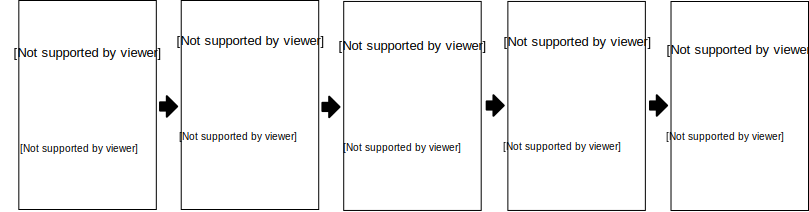
\includegraphics[scale=.75]{metodologia.pdf}}
	\caption{Etapas da Metodologia de Desenvolvimento de Pesquisa}
	\label{fig:metodologia_flow}
\end{figure}

\begin{itemize}
	\item \textbf{Pesquisa n�o sistem�tica sobre ontologias para experimentos:} foram realizado estudos n�o sistem�tico para encontrar trabalhos relacionados descrevendo ontologias para experimentos de ES e avalia��o de ontologia. Alguns estudos encontrados serviram de apoio a essa pesquisa, est�o descritos na Se��o \ref{sec:trabalhos_relacionados} ;
	
	\item \textbf{Desenvolvimento do projeto de ontologia para OntoExper-SPL:} trata sobre desenvolvimento da OntoExper-SPL, que incluiu realizar a escolha das tecnologias e ferramenta de constru��o de ontologia, como por exemplo o Prot�g�, envolver os \textit{stakeholders} no projeto com experi�ncia no dom�nio de experimenta��o, selecionar abordagens e modelos de ontologias relacionados, prototipa��o e diagrama��o do projeto;
	
	\item \textbf{Desenvolvimento do programa automatizado para povoar OntoExper-SPL:} refere-se ao processo de desenvolvimento do programa automatizado de povoamento da ontologia. Para isso foi necess�rio o uso de ferramentas, bibliotecas e linguagens de programa��o. Foram mais de 200 experimentos encontrados na literatura. Em seguida foi executado o programa de extra��o de dados, povoando a ontologia por meio dos metadados mais o programa de extra��o;
	
	\item \textbf{Avalia��o da qualidade e viabilidade do modelo:} refere-se ao estudo quali/quanti, com objetivo de avaliar a qualidade da OntoExper-SPL. Para isso foi elaborado um question�rio com oito crit�rios de qualidade, enviado para especialistas responderem, e posteriormente realizada uma an�lise estat�stica das respostas, bem como pontos de melhorias encontrados durante a avalia��o;
	
	\item \textbf{Desenvolvimento do prot�tipo de sistema de recomenda��o como prova de conceito:} ap�s processar os indiv�duos na OntoExper-SPL. Foi elaborado como prova de conceito, um prot�tipo de sistema de recomenda��o utilizando o modelos de recomenda��o \textit{Collaborative Filtering}, al�m de \textit{frameworks} e linguagens de programa��o.
\end{itemize}


\section{Organiza��o do texto}

Este cap�tulo apresentou a contextualiza��o desta disserta��o, a motiva��o e a justificativa, objetivos e metodologia. O restante da disserta��o est� estruturado da seguinte forma: o Cap�tulo \ref{sec:fundamentacao_teorica} apresenta a Fundamenta��o Te�rica sobre LPS, experimentais e quasi-experimentos em ES, qualidade de experimentos e quasi-experimentos em ES, Ontologias e Sistemas de Recomenda��o; o Cap�tulo \ref{sec:ontologia} apresenta uma Ontologia para Experimentos em LPS - OntoExper-SPL, destacando desde a concep��o ao povoamento da ontologia proposta e uma pr�-an�lise de pontos de falha da ontologia; o Cap�tulo \ref{sec:avaliacao} apresenta uma avalia��o quantitativa sobre a qualidade da OntoExper-SPL por especialistas da �rea; o Cap�tulo \ref{sec:recsys} apresenta um sistema de recomenda��o para experimentos em LPS, usando como modelo de dados a OntoExper-SPL; e o Cap�tulo \ref{sec:conclusao} apresenta as considera��es finais acerca deste projeto de disserta��o de mestrado, bom como as suas contribui��es, limita��es e trabalhos futuros.


	% ico 2
	\chapter{Revis�o de literatura}
\label{sec:revisao}


Neste t�pico � feita a revis�o de alguns conceitos sobre ...


\section{Conceitos b�sicos}
\label{sec:conc_basicos}

Em um problema...

\subsection{\textit{Iterated Local Search}}

A metaheur�stica \textit{Iterated Local Search - ILS} ...

O algoritmo \ref{alg:ILS_framework} esbo�a um pseudoc�digo do m�todo \textit{ILS}.

%Modelo de algoritmo usando clrscode3e.sty do Cormen
\begin{algorithm}
	\caption{\textit{Framework} da metaheur�stica \textit{ILS}}
	\label{alg:ILS_framework}
	\begin{codebox}
		\Procname{$\proc{Iterated-Local-Search}()$}
			\li $\id{Z_0} \gets \proc{Generate-Initial-Solution}()$
			\li $\id{Z^*} \gets \proc{Local-Search}(Z_0)$	
			\li \Repeat
				\li $\id{Z^\prime} \gets \proc{Perturbation}(Z^*)$
				\li $\id{Z^{*\prime}} \gets \proc{Local-Search}(Z^\prime)$
				\li $\id{Z^*} \gets \proc{Acceptance-Criterion}(Z^*,Z^{*\prime})$
			\li \Until ($stop~criterion~met$)
			\li \Return $Z^*$
\end{codebox}
\end{algorithm}
	
	% ico 3
	%\chapter{Proposta de Dissertação}
\label{sec:prop_sis_rec_exp}

Este capítulo apresenta a motivação, os objetivos, a metodologia, trabalhos preliminares, o empacotamento, a avaliação, as contribuições esperadas e o cronograma para o desenvolvimento desta proposta de dissertação de mestrado.

\section{Motivação}
\label{sec:moti}
Realizar um experimento em LPS exige alguns pontos de atenção específicos para garantir a qualidade do experimento. Estes pontos tem sido investigados em um trabalho de mestrado em andamento do nosso Grupo de pesquisa em Reuso Sistemático de Software e Experimentação (GRSSE), neste trabalho vem sendo elaborado diretrizes para a determinar a qualidade de experimentos em LPS. Esta tarefa possui um árduo trabalho para garantir que, aspectos específicos do domínio como, por exemplo, os artefatos utilizados que são, os objetos experimentais, a complexidade do treinamento, a dificuldade de seleção de participantes qualificados em LPS e a falta de repositórios de LPS, não influenciem nos experimentos ao ponto de invalidá-los. A falta de experimentos com qualidade afeta diretamente a possibilidade de repetição dos estudos em LPS.

Sabendo que para realizar um experimento em LPS com qualidade exige-se seguir alguns modelos e diretrizes, construir um sistema de recomendação que recomende métodos, processos, diretrizes, entre outros, para realizar um experimento em LPS, pode proporcionar facilidade ao desenvolvimento dos mesmos, incentivando a cultura e desenvolvimento de experimentos na academia e industria.

Por meio do GRSSE, foi encontrada uma lacuna nas pesquisas de qualidade em experimentos de ES em LPS que proporciona esta pesquisa, apresentando um campo aberto à pesquisa para determinar qualidade e recomendação para experimentos em LPS.


\section{Objetivos}
\label{sec:obj}

Esta pesquisa tem como objetivo geral especificar e implementar um sistema de recomendação para experimentos em LPS caracterizados por sua qualidade

Os objetivos específicos deste projeto são:

\begin{itemize}
	\item gerar e representar um conjunto de meta dados a partir das informações sobre experimentos em LPS;
	\item definir técnicas de recomendação com base nos meta dados;
	\item projeto e desenvolvimento do sistema de recomendação e;
	\item avaliar e empacotar o sistema de recomendação.
\end{itemize}

\section{Metodologia}
\label{sec:meto}

O processo de execução deste trabalho para chegar ao objetivo será, pesquisar de maneira exploratória um modelo de sistema de recomendação em experimentos de LPS. Para tal resultado será desenvolvido um projeto de software e em seguida executado o mesmo. A \ref{fig:metodologia_flow} apresenta as etapas de desenvolvimento desta pesquisa.

\begin{figure}[htb]
	\centering					
	{\includegraphics[scale=.4]{metodologia_flow.png}}
	
	\caption{Etapas da Metodologia de Desenvolvimento de Pesquisa}
	\label{fig:metodologia_flow}
\end{figure}

Neste projeto de pesquisa vamos levantar uma base de dados sobre a qualidade de experimentos em LPS. Por meio desta base será possível gerar um modelo de dados baseado em ontologias, \textbf{TBox} e \textbf{ABox}, com o objetivo de extrair informações preditivas desta base. Após processar essas informações baseada nos meta dados de qualidade de experimentos em LPS, será possível criar um sistema de recomendação, utilizando as ferramentas apropriadas de recomendação em ES.

\begin{itemize}
	\item \textbf{O Papel da Ontologia:} será de estruturar e modelar a base de informações extraída do Mapeamento Sistemático de experimentos em LPS que está sendo desenvolvido pelo GRSSE. Pode se dizer que este modelo será o conjunto de meta dados;
	
	\item \textbf{O Papel do Sistema de Recomendação:} será de interagir com o usuário afim de extrair informações relevantes, de modo que se possa determinando o deste perfil do usuário, para que possa ser realizada inferências no modelo ontológico de diretrizes de qualidade gerando recomendações de métodos, processos, diretrizes para o experimento do usuário.
\end{itemize}

O desenvolvimento do projeto, inclui realizar a escolha das tecnologias a serem usadas como ferramenta de construção do software, como por exemplo, as linguagens de programação, o ambiente de desenvolvimento, a diagramação do projeto, os \textit{stakeholders} envolvidos no projeto, ferramentas de \textit{Application Lifecycle Management} (ALM) aplicadas ao escopo do projeto, escolha das abordagens de sistemas de recomendação, definição do modelo de ontologias, definição da base de dados para representação tanto, dos dados de origem (itens, usuários), quanto, para representação dos dados para apresentação e armazenamento dos resultados obtidos da recomendação. 

Após a definição do projeto de software, inicia-se o processo de desenvolvimento do sistema de recomendação. Com o auxílio de ferramentas de ALM será possível acompanhar por todos os \textit{stakeholders} envolvidos o desenvolvimento online da ferramenta, desta forma se tornando um processo mais colaborativo entre eles. Inicialmente será realizado a modelagem dos dados extraído da avaliação de qualidade dos experimentos em LPS realizado pelo trabalho do GRSSE, que são 174 experimentos encontrado na literatura nesse ramo de pesquisa. Em seguida será aplicado um modelo de ontologia definido no projeto de software, nesta base de informações de experimentos, tem como propósito, realizar predições para um modelo mais abstrato sobre qualidade de experimentos em LPS. Na sequência será desenvolvido o modelo de recomendação, este desenvolvimento consiste na modelagem dos dados encontrado na predição da ontologia para extrair as informações necessárias para o modelo de recomendação, posteriormente aplicar os algoritmos neste modelo. Em seguida será desenvolvido um \textit{front-end} de interação com o usuário poder dar entrada na informações iniciais para gerar as recomendações. O último passo será realizado um estudo para avaliação deste sistema de recomendação.

\begin{figure}[htb]
	\centering					
	{\includegraphics[scale=.5]{RSSE-overview.png}}
	
	\caption{Modelagem geral da RSSE proposta}
	\label{fig:RSSE-overview}
\end{figure}

A \ref{fig:RSSE-overview} apresenta o conceito geral da metodologia deste projeto. Iniciando pela entrada dos usuários, depois extraímos as preferencias dele, e em seguida será feita a extração de informações de contexto utilizando a base de meta dados em LPS, para então fazer inferência nos itens (que são experimentos em LPS), por meio dessa inferência será obtido as recomendações.

Inicialmente, a entrada de dados dos usuários está sendo definido da seguinte forma:

\begin{itemize}
	\item Informações de LPS:
		\subitem Dominio;
		\subitem Sub-dominio;
		\subitem Tipos de artefatos e;
		\subitem Feature module.
	\item Experimentos
		\subitem filtrar por qualidade.
\end{itemize}


\section{Trabalhos Preliminares}

\subsection{Transformação de planilha para banco de dados}

A extração de dados a partir da planilha de Excel da revisão sistemática do GRSSE. Para esta transformação está sendo utilizando uma ferramenta de ETL (\textit{Extract, Transform, Load}) chamada PDI (\textit{Pentaho Data Integration}) transportando os dados da planilha para um banco de dados relacional (MySql).

A \ref{fig:etl-meta-dados} do Apêndice \ref{apen:a1}, apresenta o esta transformação em construção, este processo é realizado por meio de uma leitura linha-a-linha da planilha e persistindo em uma tabela na base de dados MySql previamente definida.

\subsection{Grafo inicial de diretrizes para base ontológica de qualidade de experimentos em LPS}

Para levantar as diretrizes iniciais da ontologia (\textbf{TBox} e \textbf{ABox}), está sendo desenvolvido um grafo usando uma ferramenta de mapa mental (Xmind), mapeando as possíveis classificações e suas tipagens bem como alguns exemplos de informações inerentes aos domínios classificados.

Esta construção inicial pode ser visto na \ref{fig:diretrizes-01} do Apêndice \ref{apen:a3}, e com exemplos iniciais na \ref{fig:diretrizes-03} do Apêndice \ref{apen:a3}. Para concluir esta etapa falta filtrar as classes que realmente representam uma relevância para qualidade em LPS e cria os relacionamento entre estas classes de domínios.

\subsection{SQL para listar diretrizes comuns}
Para auxiliar na extração de informações das classificação de domínio da ontologia, foi desenvolvidos sete \textit{querys} (como pode ser visto no Apêndice \ref{apen:a2}) para formar uma base inicial de dados (\textbf{ABox}) do nosso modelo ontológico.


\section{Empacotamento}

Todo projeto está sendo versionado no Github pelo link: https://github.com/rickvig/pcc-pesquisa.


\section{Avaliação}
\label{sec:aval}
Na Literatura é possível encontrar algumas dimensões para avaliação de RSSE, e as recomendações providas por ele. Em \citet{robillard2010recommendation} são apresentadas 16 dimensões de avaliação para um RSSE, que estão apresentadas na \ref{tab:dimensoes}. Cada dimensão possui sua técnica de avaliação, algumas são quantitativas outras qualitativas, algumas possuem as duas abordagens.

\begin{table}[]
	\centering
	\caption{Dimensões de avaliação para RSSE. Tradução de \citet{robillard2010recommendation}}
	\label{tab:dimensoes}
	\begin{tabular}{|l|l|l|ll}
		\cline{1-3}
		\multicolumn{1}{|c|}{\cellcolor[HTML]{C0C0C0}\textbf{Dimensão}} & \multicolumn{1}{c|}{\cellcolor[HTML]{C0C0C0}\textbf{Descrição}} & \multicolumn{1}{c|}{\cellcolor[HTML]{C0C0C0}\textbf{Tipo de métrica}} &  &  \\ \cline{1-3}
		Corretude & \begin{tabular}[c]{@{}l@{}}Quão próximo é a recomendação do \\ conjunto de recomendações que \\ assumimos ser corretas?\end{tabular} & quantitativa &  &  \\ \cline{1-3}
		Cobertura & \begin{tabular}[c]{@{}l@{}}Até que ponto a cobertura do SR sobre \\ um conjunto de itens ou o espaço do usuário?\end{tabular} & quantitativa &  &  \\ \cline{1-3}
		Diversidade & Qual a diversidade das recomendações? & quantitativa &  &  \\ \cline{1-3}
		Confiável & Como a recomendação pode ser confiável? & qualitativa &  &  \\ \cline{1-3}
		Confiança do SR & Quão confiante o SR é? & \begin{tabular}[c]{@{}l@{}}quantitativa / \\ qualitativa\end{tabular} &  &  \\ \cline{1-3}
		Novidade & \begin{tabular}[c]{@{}l@{}}Qual é o sucesso do SR em gerar novas \\ recomendações ou recomendações ainda \\ desconhecidas para o usuário?\end{tabular} & \begin{tabular}[c]{@{}l@{}}quantitativa / \\ qualitativa\end{tabular} &  &  \\ \cline{1-3}
		Acaso & \begin{tabular}[c]{@{}l@{}}Até que ponto o SR ainda promove \\ surpresa com sucesso?\end{tabular} & \begin{tabular}[c]{@{}l@{}}quantitativa /\\ qualitativa\end{tabular} &  &  \\ \cline{1-3}
		Utilidade & \begin{tabular}[c]{@{}l@{}}Qual é o ganho de valor dessa \\ recomendação para o usuário?\end{tabular} & \begin{tabular}[c]{@{}l@{}}quantitativa / \\ qualitativa\end{tabular} &  &  \\ \cline{1-3}
		Risco & \begin{tabular}[c]{@{}l@{}}Qual é o risco para o usuário \\ aceitar essa recomendação?\end{tabular} & qualitativa &  &  \\ \cline{1-3}
		Robustez & \begin{tabular}[c]{@{}l@{}}Qual é a tolerância do SR para um \\ viés ou uma informação falsa?\end{tabular} & quantitativa &  &  \\ \cline{1-3}
		\begin{tabular}[c]{@{}l@{}}Taxa de \\ Aprendizagem\end{tabular} & \begin{tabular}[c]{@{}l@{}}Quão rápido é o SR para adicionar novas \\ informações ou atualizar a lista de recomendação?\end{tabular} & quantitativa &  &  \\ \cline{1-3}
		Usabilidade & \begin{tabular}[c]{@{}l@{}}O qual usável é o SR? Será fácil dos \\ usuários se adequar de uma forma apropriada?\end{tabular} & \begin{tabular}[c]{@{}l@{}}quantitativa / \\ qualitativa\end{tabular} &  &  \\ \cline{1-3}
		Escalabilidade & \begin{tabular}[c]{@{}l@{}}Quão escalável é o SR em relação \\ ao numero de usuários, levando em \\ consideração o tamanho dos dados e \\ a performance dos algoritmos?\end{tabular} & quantitativa &  &  \\ \cline{1-3}
		Estabilidade & Quão consistente é o SR em um período de tempo? & quantitativa &  &  \\ \cline{1-3}
		Privacidade & Existe algum risco a privacidade do usuário? & \begin{tabular}[c]{@{}l@{}}quantitativa / \\ qualitativa\end{tabular} &  &  \\ \cline{1-3}
		\begin{tabular}[c]{@{}l@{}}Preferência do\\ Usuário\end{tabular} & Como o usuário entende o SR? & \begin{tabular}[c]{@{}l@{}}quantitativa / \\ qualitativa\end{tabular} &  &  \\ \cline{1-3}
	\end{tabular}
\end{table}

\begin{table}[]
	\centering
	\caption{Categorização das 16 dimensões. Tradução de \citet{robillard2010recommendation}}
	\label{tab:dimens-catg}
	\begin{tabular}{@{}llll@{}}
		\toprule
		\begin{tabular}[c]{@{}l@{}}Centralizado na \\ Recomendação\end{tabular} & \begin{tabular}[c]{@{}l@{}}Centralizado no \\ Usuário\end{tabular} & \begin{tabular}[c]{@{}l@{}}Centralizado no \\ Sistema\end{tabular} & \begin{tabular}[c]{@{}l@{}}Centralizado na \\ Entrega\end{tabular} \\ \midrule
		Corretude & Confiável & Robustez & Usabilidade \\
		Cobertura & Novidade & Taxa de Aprendizagem & Preferência do usuário \\
		Diversidade & Acaso & Escalabilidade &  \\
		Confiança do SR & Utilidade & Estabilidade &  \\
		& Risco & Privacidade &  \\ \bottomrule
	\end{tabular}
\end{table}

Essas dimensões podem ser subdivididas em categorias como mostra a \ref{tab:dimens-catg}. As dimensões centradas na recomendação avaliam principalmente as recomendações geradas pelo próprio sistema de recomendação. As dimensões centradas no usuário nos permitem avaliar se o sistema de recomendação atende às necessidades do seu usuário final. As dimensões centradas no sistema, em contraste a dimensões anterior, estas fornecem principalmente formas de avaliar o próprio sistema de recomendação ao invés das recomendações. Finalmente, as dimensões centradas na entrega estão focadas principalmente no contexto de uso do sistema de recomendação \cite{robillard2010recommendation}.

\begin{figure}[htb]
	\centering					
	{\includegraphics[scale=.4]{rel_metricas_pt.png}}
	
	\caption{Cruzamento de interesses entre as dimensões. Traduzido e adaptado de \citet{robillard2010recommendation}}
	\label{fig:rel_metricas}
\end{figure}

A \ref{fig:rel_metricas} apresenta o relacionamentos direto e adverso entro as métricas de avaliação. Por exemplo, o relacionamento direto entre as métricas Corretude e Cobertura, significa que, se o RSSE possui a métrica Corretude  provavelmente terá a métrica de Cobertura. No caso do relacionamento adverso, por exemplo, as métricas Corretude e Diversidade, significa que, se o RSSE possui a métrica Corretude provavelmente não terá a métrica Diversidade


\section{Contribuições Esperadas}
\label{sec:contr}

Espera-se que com este trabalho seja encontrado um modelo (projeto e implementação) de recomendação para experimentos de LPS. Espera-se também realizar um estudo de caso a fim de analisar o modelo proposto.

Espera-se que com esta pesquisa se inicie um processo de melhoramento na qualidade de experimentação em LPS, em que, possa ser realizado por meio deste projeto e implementação de sistema de recomendação.

Contribuir com a comunidade de LPS a projetar e executar experimentos melhores, desta forma aumentar a confiança do corpo de conhecimento visando a transferência de tecnologia para indústria.

\section{Cronograma}
\label{sec:cron}

As etapas que compõem o cronograma de execução desta proposta de projeto de dissertação de mestrado são descritas a seguir e apresentadas abaixo na \ref{fig:cronograma}, evidenciado as que estão em andamento a serem executadas e concluídas de acordo com legenda.

\begin{itemize}
	\item E1 - Revisão da Literatura
	\item E2 - Projeto: Tecnologias
	\item E3 - Projeto: Modelo de Ontologias
	\item E4 - Projeto: Modelo de Predição
	\item E5 - Projeto: Modelagem de dados
	\item E6 - Projeto: Modelo de Recomendação
	\item E7 - Projeto: Front-End
	\item E8 - Desenvolvimento: Ontologias
	\item E9 - Desenvolvimento: Predição
	\item E10 - Desenvolvimento: Recomendação
	\item E11 - Desenvolvimento: Front-End
	\item E12 - Testes
	\item E13 - Avaliação dos Resultados
	\item E14 - Escrever Qualificação
	\item E15 - Defesa da Qualificação
	\item E16 - Escrever Dissertação
	\item E17 - Defesa da Dissertação
	\item E18 - Escrita de artigos para conferencia e periódicos qualificados
\end{itemize}

\begin{figure}[]
	\centering					            
	{\includegraphics[scale=.45]{cronograma.png}}
	
	\caption{Cronograma de desenvolvimento da pesquisa - Anos 2018/2019}
	\label{fig:cronograma}
\end{figure}

	
	% ico 4
	\chapter{Uma Ontologia para Experimentos em LPS - OntoExper-LPS}
\pagestyle{plain}
\label{sec:ontologia}


\section{Considera��es Iniciais}
\label{sec:concidaracoes_iniciais}

Este cap�tulo apresenta a elabora��o da proposta de ontologia OntoExper-LPS, sua concep��o, a constru��o do projeto, exemplos de aplica��o, uma breve avalia��o emp�rica e considera��es finais. Dessa forma a estrutura deste cap�tulo fica, na Se��o \ref{sec:concepcao} apresenta o processo de concep��o do modelo seguindo a tipologia de \cite{almeida2003visao} bem como a elabora��o de um grafo como modelagem inicial da ontologia, seguindo como base um modelo conceitual clusterizado sobre elementos experimentais de ES em LPS; na Se��o \ref{sec:projeto} foi desenvolvido o projeto da OntoExper-LPS para se obter modelo ontol�gico, foi utilizado como tecnologia base OWL (\textit{Ontology Web Language}) juntamente com a Ferramenta Prot�g�, o resultado final foi um artefato do tipo OWL contendo toda modelagem de classes, subclasses, propriedades de objeto e propriedades dos dados, al�m da modelagem, foi criado nesta se��o, um programa automatizado para povoar a ontologia utilizando os metadados levantados pelo GReater, este programa conta com a utiliza��o da linguagem de programa��o Python e a biblioteca OwlReady2; na Se��o \ref{sec:exemplo} foi elaborado uma consulta SPARQL para demonstrar como interagir com a ontologia e uma breve explica��o deste procedimento; na Se��o \ref{sec:avaliacao_empirica} foi realizado uma avalia��o emp�rica do modelo, por meio da ferramenta OOPS! que avalia pontos de falha do modelo, nesta se��o discutimos como estes ponto de falham impacta no modelo proposto por este trabalho.


\section{Concep��o}
\label{sec:concepcao}

Com base na tipologia proposta por \cite{almeida2003visao} definimos o tipo da ontologia proposto neste trabalho, descrito na Tabela \ref{tab:tipo-modelo-ontologia}. Todas as tipologias para ontologias podem ser encontradas no Ap�ndice \ref{apendice:a-tipologia}

Ou seja, podemos tipificar o modelo proposto como; \textbf{quanto � fun��o:} � uma ontologia de dom�nio, \textbf{quanto ao grau de formalismo:} � uma ontologia semi formal, \textbf{quanto � aplica��o:} � uma ontologia de especifica��o, \textbf{quanto � estrutura:} � uma ontologia de dom�nio e \textbf{quanto ao conte�do:} � tanto uma ontologia para modelagem de conhecimento quanto para aplica��o de dom�nio.

Tamb�m foi aplicado o seguinte processo de elabora��o da ontologia, seguindo os processos proposto por \cite{fernanda2007modelagem}:

\begin{itemize}
	\item Defini��o e estrutura��o dos termos por meio de classes;  
	\item Estabelecimento de propriedades (atributos) inerentes ao conceito representado por um termo;
	\item Povoamento da estrutura que satisfa�am um conceito e as suas propriedades;  
	\item Estabelecimento de rela��es entre os conceitos;
	\item Elabora��o de senten�as para restringir infer�ncias de conhecimento baseadas na estrutura.
\end{itemize}

\begin{landscape}
	\topskip0pt
    \vspace*{\fill}
	\begin{table}[]
		\label{tab:tipo-modelo-ontologia}
		\caption{Tipagem da ontologia proposta}
		\centering
		\begin{tabular}{@{}lll@{}}
			\toprule
			Abordagem & Classifica��o & Descri��o \\ \midrule
			\begin{tabular}[c]{@{}l@{}}Quanto � fun��o \\ Mizoguchi; Vanwelkenbuyse \\ n; Ikeda (1995)\end{tabular} & Ontologias de dom�nio & \begin{tabular}[c]{@{}l@{}}Reutiliz�veis no dom�nio, fornecem vocabul�rio \\ sobre conceitos e seus relacionamentos, sobre as \\ atividades e regras que os governam.\end{tabular} \\
			\begin{tabular}[c]{@{}l@{}}Quanto ao grau de formalismo \\ Uschold; Gruninger (1996)\end{tabular} & Ontologias semi informais & \begin{tabular}[c]{@{}l@{}}Expressa em linguagem natural de forma restrita \\ e estruturada.\end{tabular} \\
			\begin{tabular}[c]{@{}l@{}}Quanto � aplica��o \\ Jasper; Uschold (1999)\end{tabular} & \begin{tabular}[c]{@{}l@{}}Ontologias como \\ especifica��o\end{tabular} & \begin{tabular}[c]{@{}l@{}}Cria-se uma ontologia para um dom�nio, a qual � \\ usada para documenta��o e manuten��o no \\ desenvolvimento de softwares.\end{tabular} \\
			\begin{tabular}[c]{@{}l@{}}Quanto � estrutura \\ Haav; Lubi (2001)\end{tabular} & Ontologias de dom�nio & \begin{tabular}[c]{@{}l@{}}Descrevem o vocabul�rio relacionado a um dom�nio, \\ como, por exemplo, medicina ou autom�veis\end{tabular} \\
			\multirow{3}{*}{\begin{tabular}[c]{@{}l@{}}Quanto ao conte�do \\ Van-Heijist; Schreiber; \\ Wielinga (2002)\end{tabular}} & \begin{tabular}[c]{@{}l@{}}Ontologias de modelagem\\ do conhecimento\end{tabular} & \begin{tabular}[c]{@{}l@{}}Especificam conceitua��es do conhecimento, t�m uma \\ estrutura interna semanticamente rica e s�o refinadas\\ para uso no dom�nio do conhecimento que descrevem\end{tabular} \\
			& Ontologias de aplica��o & \begin{tabular}[c]{@{}l@{}}Cont�m as defini��es necess�rias para modelar o \\ conhecimento em uma aplica��o.\end{tabular} \\
			& Ontologias de dom�nio & \begin{tabular}[c]{@{}l@{}}Expressam conceitua��es que s�o espec�ficas para \\ um determinado dom�nio do conhecimento.\end{tabular} \\ \bottomrule
		\end{tabular}
	\end{table}
	\vspace*{\fill}
\end{landscape}

O primeiro passo foi desenvolver um grafo como modelo inicial da ontologia OntoExper-LPS, o objetivo principal foi de externalizar id�ias iniciais do modelo e visualizar hierarquias e relacionamentos entre os termos inicialmente propostos.

\begin{figure}[]
	\centering 
	\includegraphics[scale=0.5]{grafo-inicial.pdf}
	\caption{Grafo inicial da proposta de ontologia.}
	\label{figure:graph-all-class}
\end{figure}

A \ref{figure:graph-all-class} representa este modelo inicial contendo a defini��o principal dos termos para o experimento, Experimento SPL, Documenta��o, Template, Avalia��o, Discuss�o, An�lise, Execu��o e Planejamento. Em seguida evolu�mos para poss�veis termos de mais baixa hierarquia, que est�o definidas a seguir:


\begin{itemize}
	\item Documenta��o;
	\begin{itemize}
		\item Dom�nio em LPS;
		\item \textit{Abstract}:
		\begin{itemize}
			\item Palavra Chave; 
			\item Limita��es;
			\item Conclus�es;
			\item Resultados;
			\item M�todos; e
			\item Objetivos.			
		\end{itemize}
		\item Introdu��o:
		\begin{itemize}
			\item Contexto;
			\item Objetivo da Pesquisa (GQM); e
			\item Quest�es do Problema.
		\end{itemize}
		\item Trabalhos Relacionados:
		\begin{itemize}
			\item Estudos Relacionados;
			\item Tecnologia sob Investiga��o;
			\item Tecnologia Alternativa; e
			\item Relev�ncia na Pr�tica.
		\end{itemize} 
		\item Template:
		\begin{itemize}
			\item Observa��o.
		\end{itemize}
		\item Refer�ncias;
		\item Agradecimentos;
		\item Conclus�o; e
		\item Ap�ndice.
	\end{itemize}
	\item Planejamento:
	\begin{itemize}
		\item Contexto:
		\begin{itemize}
			\item Local.
		\end{itemize} 
		\item Unidade Experimental:
		\begin{itemize}
			\item Sele��o dos Participantes;
		\end{itemize} 
		\item Material Experimental:
		\begin{itemize}
			\item Artefatos de SPL;
			\begin{itemize}
				\item Fonte
			\end{itemize} 
		\end{itemize} 
		\item Projeto Experimental;
		\item Par�metros;
		\item Vari�veis;
		\item Procedimentos;
		\item Objetivo;
		\item Hip�teses;
		\item Tarefas;
		\item An�lises de procedimentos;
	\end{itemize} 
	\item Execu��o:
	\begin{itemize}
		\item Prepara��o:
		\begin{itemize}
			\item Projeto Piloto;
		\end{itemize}	 
		\item Execu��o; e
		\item Desvio do Planejamento;
	\end{itemize}
	\item An�lise:
	\begin{itemize}
		\item Tipo de An�lise:
		\begin{itemize}
			\item Meta An�lise
			\item Tipo de An�lise de Hip�tese;
		\end{itemize} 
		\item Teste de Hip�tese:
		\begin{itemize}
			\item P-value
		\end{itemize} 
		\item Estat�stica Descritiva;
		\item An�lise qualitativa;
		\item Prepara��o do \textit{Dataset};
	\end{itemize} 
	\item Discuss�o:
	\begin{itemize}
		\item Amea�as a Validade:
		\begin{itemize}
			\item Amea�a a Validade em LPS.
		\end{itemize} 
		\item Avalia��o dos Resultados;
		\item Infer�ncias;
		\item Li��es Aprendidas;
	\end{itemize}	 
	\item Empacotamento:
	\begin{itemize}
		\item Pacote Experimental.
	\end{itemize} 
	\item Avalia��o:
	\begin{itemize}
		\item Abordagem de Avalia��o.
	\end{itemize} 

\end{itemize}

Esta modelagem inicial da ontologia foi baseada no trabalho de mapeamento sistem�tico de experimentos em LPS de \cite{Furtado2018}, por meio de uma an�lise explorat�ria dos dados levantados nesse mapeamento, foi poss�vel usa-lo como guia de informa��es e metadados de ESE em LPS.

O mapeamento sistem�tico levou em considera��o o temple experimental de Wohlin, que traz cinco fases para elabora��o de ESE, s�o eles, Defini��o, Planejamento, Opera��o, An�lise e Interpreta��o \cite{wohlin2012}.

\begin{landscape}
	\topskip0pt
    \vspace*{\fill}
	\begin{figure}[]
		\centering 
		\includegraphics[scale=.65]{modelo-conceitual-clusterizado.pdf}
		\caption{Modelo Conceitual Clusterizado.}
		\label{figure:conceptual_model_clustering}
	\end{figure}
	\vspace*{\fill}
\end{landscape}

A \ref{figure:conceptual_model_clustering}, apresenta uma modifica��o do modelo conceitual original, elaborada no trabalho de \cite{Furtado2018}, onde foi aplicado a clusteriza��o separando cada cluster para cada fase do template experimental de Wohlin. Esta clusteriza��o foi necess�ria para compreens�o mais abstrata das rela��es entre os termos do dom�nio levantados no modelo conceitual original e as fases do template do Wholin. Dessa forma foi poss�vel validar cada termo do grafo inicialmente proposto.
	
Em seguida, um diagrama de classes foi elaborado para representar de uma maneira mais intuitiva a modelagem inicial, realizada com grafos. O objetivo � transformar cada termos do grafo em uma classe do conceito de Orienta��o a Objetos. Nessa representa��o, a modelagem da \textit{TBox}, ou seja, a rela��o entre os termos (classes) e suas propriedades (atributos) ficou mais clara. Essa forma de representa��o destacou a rela��o principal quando definimos a composi��o da classe Experiment e ExperimentSPL em quase todas as outras subclasses. Nesta representa��o tamb�m ficou expl�cita a tipifica��o das propriedades, para posteriormente executar a inser��o da \textit{ABox} na modelagem.

A \ref{figure:class_diagram_ontology} apresenta o diagrama de classe gerado para o modelagem da ontologia. Este diagrama representa todas composi��es de classes que existe com Experiment e ExperimentSPL, bem como as rela��es hier�rquicas como por exemplo, ExperimentSPL � uma subclasse de Experiment.

\begin{landscape}
	\topskip0pt
    \vspace*{\fill}
	\begin{figure}[]
		\centering
		\includegraphics[scale=.3]{class-diagram-ontology.png}
		\caption{Diagrama de Classe para proposta da modelagem da ontologia.}
		\label{figure:class_diagram_ontology}
	\end{figure}
	\vspace*{\fill}
\end{landscape}

Posteriormente, foi utilizada a ferramenta Prot�g� para constru��o oficial da ontologia, seguindo os padr�es OWL.


\section{Projeto}
\label{sec:projeto}

Definimos a cria��o da ontologia usando a tecnologia OWL, foram constru�das as classes e subclasses para representar os elementos da ontologia, por meio da ferramenta Prot�g�.

\subsection{Modelagem com Prot�g�}
\label{sec:protege}

A ferramenta Prot�g� � um ambiente de desenvolvimento voltado para cria��o de ontologias. Ela disp�e de uma interface gr�fica para edi��o de ontologias e uma arquitetura para a cria��o de ferramentas baseadas em conhecimento. Pode ser usada tanto por, desenvolvedores de sistema, como por especialistas em dom�nio, para criar bases de conhecimento, permitindo representar facilmente o conhecimento de uma �rea. Este editor � capaz de tratar classes, com sua defini��o e exemplos, simultaneamente propriedades de objetos e de dados \cite{DBLP:journals/aimatters/Musen15}.

% O padr�o OWL foi usado no OntoExper-LPS para definir todos os elementos, classes, propriedades de objetos e dados.

Fazendo uma analogia ao diagrama de classe, no Prot�g�, as classes, os atributos de classes e seus relacionamentos est�o em um contexto de entidades. As classes e hierarquias s�o definidos na aba \textbf{Classes}, os relacionamentos s�o definidos na aba \textbf{Propriedades de Objetos} e os atributos s�o definidos na aba \textbf{Propriedade dos Dados}.

Definimos nossas entidades com base do diagrama de classe constru�do na fase de concep��o, com a seguinte estrutura (i) defini��o de classes (ii) defini��o das propriedades de objetos, (iii) defini��o das propriedades dos dados.

\subsubsection{Defini��o de classes}

No Prot�g�, definimos uma classe raiz chamada \textit{Thing} na qual todas as outras classes s�o filhas dela. A \ref{figure:class_defition_protege} apresenta a defini��o da classe Experiment dentro do modelo, neste momento a defini��o � composta pelo nome da classe e seus principais relacionamentos \textit{(Equivalent To e SubClass Of)}.

\begin{figure}[htb]
	\centering 
	\includegraphics[scale=.5]{entidades-protege.png}
	\caption{Defini��o da classe Experiment no Prot�g�.}
	\label{figure:class_defition_protege}
\end{figure}

\subsubsection{Defini��o das propriedades de objetos}

No Prot�g�, definimos uma propriedade de objeto raiz chamada \textit{topObjectProperty} na qual todas as outras propriedades s�o filhas dela. A \ref{figure:object_prop_defition_protege} apresenta a defini��o de propriedade de objeto para propriedade \textit{documentation}, neste momento a defini��o � composta pelo nome da propriedade e seus relacionamentos com classes, Dom�nio \textit{(Domains)} e Alcance \textit{(Ranges)}.

\begin{figure}[!htb]
	\centering 
	\includegraphics[scale=.5]{entidades-protege-object-properties.png}
	\caption{Defini��o da propriedade de objeto documentation no Prot�g�.}
	\label{figure:object_prop_defition_protege}
\end{figure}

\subsubsection{Defini��o das propriedades dos dados}

No Prot�g�, definimos uma propriedade de dados raiz chamada \textit{topDataProperty} na qual todas as outras propriedades s�o filhas dela. Para cada Propriedade de dado definimos um conjunto de classes de seu Dom�nio e um conjunto de tipos de dados (predefinido) de seu Alcance, por exemplo, a propriedade de dado \textit{nameSPLUsed} possui como classe de dom�nio ExperimentSPL e como alcance um \textit{xsd:string}. A \ref{figure:data_prop_defition_protege} apresenta a defini��o de propriedade de dado para chamada \textit{nameSPLUsed}, neste momento a defini��o � composta pelo nome da propriedade e seus relacionamentos, Dom�nio (uma classe) e Alcance (uma tipagem).

\begin{figure}[htb]
	\centering 
	\includegraphics[scale=.5]{entidades-protege-data-properties.png}
	\caption{Defini��o da propriedade de dado nameSPLUsed no Prot�g�.}
	\label{figure:data_prop_defition_protege}
\end{figure}

\subsubsection{Artefato gerado pelo Prot�g�}

Ao final, o Prot�g� gera um arquivo \textit{.owl} contendo toda a defini��o do modelo. A \ref{figure:graph_ontology_model} fornece uma vis�o geral no formato de grafo do projeto, contendo todas as classes. Usamos a ferramenta WebVOWL \cite{lohmann2016visualizing} para gerar essa vis�o.

\begin{figure}[htb]
	\centering 
	\includegraphics[scale=.6]{ontology-populate-valid-owl-2.pdf}
	\caption{Grafo da modelagem da ontologia - gerado pelo WbVOWL.}
	\label{figure:graph_ontology_model}
\end{figure}

\subsection{Povoamento com Python}
\label{sec:python}

A pr�xima etapa, ap�s a modelagem da ontologia, foi inserir os indiv�duos na mesma, ou seja, popular a ontologia para realiza��o de infer�ncias futuras. Apesar do Prot�g� ter capacidade para realizar essa opera��o, optamos por utilizar um script para realizar tal tarefa, visto que, no Prot�g� o processo de inserir indiv�duos na ontologia � realizado de modo manual, por meio do menu \textit{Individuals by Class}, onde � preciso selecionar propriedade por propriedade para cada indiv�duo. Sabendo que para cada indiv�duo temos 84 propriedades de dados mais 8 propriedade de objetos, somando um total de 92 relacionamentos para cada indiv�duo. Portanto, sabendo que temos aproximadamente duzentos indiv�duos a serem inseridos em uma carga inicial, seriam aproximadamente mais de 184.000 itera��es manuais no Prot�g�. Este c�lculo est� descrito na Equa��o \ref{eq:numero_iteracoes_manuais}.

\begin{equation}
	\label{eq:numero_iteracoes_manuais}
	n^{\circ}\, iteracoes\, manuais = n^{\circ}\, relacionamentos * n^{\circ}\, individuos
\end{equation}

Dado essa estimativa de opera��es manuais optamos pela utiliza��o de uma ferramenta script, a fim de facilitar e automatizar a inser��o dos indiv�duos e posteriormente a inser��o de novos indiv�duos. Escolhemos a linguagem de programa��o Python por fornecer bibliotecas prontas, tanto para manipula��o de dados em planilhas (Pandas), como para ontologia em arquivos .owl (OwlReady2), para tal finalidade.

\subsubsection{Script}

Para o ambiente de desenvolvimento do script, utilizamos outra ferramenta do Python chamada Jupyter Notebook \cite{PER-GRA:2007} para auxiliar na execu��o e valida��o de c�digo. O processo do script se assemelha a um processo de ETL \textit{(Extract Transform Load)}, onde extra�mos os dados originais da planilha, desenvolvida no trabalho de revis�o sistem�tica sobre experimentos em LPS, e manipulamos estes dados para inserir na ontologia, seguindo a modelagem inicial constru�da no Prot�g�.

Para  leitura dos dados da planilha usamos a biblioteca Pandas \cite{mckinney-proc-scipy-2010}, ela nos retorna um objeto do tipo \textit{Dataframe}, no qual � a representa��o da pr�pria planilha no ambiente de programa��o Python.

Os dados da planilha est�o estruturados na seguinte forma, cada linha representa um artigo encontrado no mapeamento sistem�tico, e cada coluna representa um dado extra�do deste artigo. Segue o mapeamento de cada coluna. 

Com rela��o ao \textit{Experiment} temos:  \textit{ID, Title, Authorship, Publication year, Publication type, Publication venue, Pages number, dados de Experimentos em SPL temos: Is it Real or Academic SPL?, SPL Name used, Was the SPL source used informed? (Y/N) (If yes, which one?)}. 

Com rela��o a \textit{Documentation} temos: \textit{Does it use template? (Y/N)?,  If yes, what template?, Observations about the template used. Para o Abstract temos: Objective (What is the question addressed with this research?), Abstract - Background (Why is this research important?), Methods (What is the statistical context and methods applied?), Results (What are the main findings? Practical implications?), Limitations (What are the weakness of this research?), Conclusions (What is the conclusion?) e Keywords. Para o Introduction Section temos: Problem statement (What is the problem? Where does it occur? Who has observed it? Why is it important to be solved?), Research objective (GQM) (What is the research question to be answered by this study?), Context (What information is necessary to understand whether the research relates to a specific situation (environment)?). Para o Related Work Section temos: Technology under investigation (What is necessary for a reader to know about the technology to reproduce its application?), Alternative technologies (How does this research relate to alternative technologies? What is the control treatment?), Related studies (How this research relates to existing research (studies)? What were the results from these studies?), Relevance to practice (How does it relate to state of the practice?). Para o Conclusions and Future Work Section temos: Summary (The purpose of this section is to provide a concise summary of the research and its results as presented in the former sections), Impact (Description of impacts with regard to cost, schedule, and quality, circumstances under which the approach presumably will not yield the expected benefit), Future Work (What other experiments could be run to further investigate the results yielded or evolve the Body of Knowledge)}.

Com rela��o ao \textit{Experiment Planning} temos: \textit{Goals (Formalization of goals, refine the important constructs of the experiment's goal), Experimental Units (From which population will the sample be drawn? How will the groups be formed (assignment to treatments)? Any kind of randomization and blinding has to be described?), Experimental Material (Which objects are selected and why?), Tasks (Which tasks have to be performed by the subjects?), Hypotheses (What are the constructs and their operationalization? They have to be traceable derived from the research question respectively the goal of the experiment), Parameters (What are the constructs and their operationalization? They have to be traceable derived from the research question respectively the goal of the experiment), Variables (What are the constructs and their operationalization? They have to be traceable derived from the research question respectively the goal of the experiment), Experiment Design (What type of experimental design has been chosen?), Procedure (How will the experiment (i.e., data collection) be performed? What instruments, materials, tools will be used and how?) Analysis Procedure (How will the data be analyzed?), Is it a quasi-experiment? (Y/N) If yes, is it explicit in the study?, Is it an Original or Replicated Experiment?,	How was the selection of participants/experimental objects? - Simple random sampling; - Systematic sampling; - Stratified random sampling; - Convenience sampling; - Quota sampling, Context of the experiment (in vivo, in vitro, ...), Design Experimental: - One factor with two treatments; - One factor with more than two treatments; - Two factors with two treatments; - More than two factors each with two treatments, SPL artifact used, Context Selection (Off-line vs. on-line, Student vs. professional, Toy vs. real problems, Specific vs. general)}.

Com rela��o a \textit{Execution (Operation)} temos: \textit{Preparation (What has been done to prepare the execution of the experiment (i.e., schedule, training), Deviations from the Plan (Describe any deviations from the plan, e.g., how was the data collection actually performed?), The pilot project was carried out? (Y/N) If Yes, how many?}.

Com rela��o a \textit{Analysis (Analysis and Interpretation)} temos: \textit{Descriptive statistics (What are the results from descriptive statistics?), Data set preparation (What was done to prepare the data set, why, and how?), Hypothesis testing (How was the data evaluated and was the analysis model validated?), Do it have qualitative analysis of the experiment? (Y/N), If yes, what qualitative analysis was performed?, How the data has been analyzed? (Ex: Correlation, Hypothesis Test, meta-analysis), Is the conclusion of the experiment analysis based on P-value? (Y/N), Did the study perform meta-analysis? (Y/N)}.

Com rela��o a \textit{Discussion} temos: \textit{Evaluation of Results and Implications (Explain the results and the relation of the results to earlier research, especially those mentioned in the Background section), Threats to Validity (How is validity of the experimental results assured? How was the data actually validated?) (Follow are the 4 threats proposed by Wohlin: internal, external, construct and conclusion? (Y/N)), Inferences (Inferences drawn from the data to more general conditions), Lessons learned (Which experience was collected during the course of the experiment), Threats to validity in SPL}.

Com rela��o a \textit{Evaluation} temos: \textit{The authors were concerned with evaluating the quality of the experiments? (Y/N)}.

Com rela��o a \textit{Package} temos: \textit{Is the experimental package informed? (Y/N) (If yes, what URL? And the link is still available? (Y/N))}

Outros dados: \textit{Acknowledgements Section (Sponsors, participants, and contributors who do not fulfil the requirements for authorship should be mentioned), References Section (All cited literature has to be presented in the format requested by the publisher, Appendices Section (Experimental materials, raw data, and detailed analyses, which might be helpful for others to build upon the reported work should be provided)}.

\subsubsection{Manipula��o dos Dados}

Para inserir os indiv�duos na OntoExper-LPS, foi preciso manipular os dados da planilha com as seguintes opera��es.

\textbf{Primeira opera��o:} separa��o \textit{(split)} de dados de uma �nica coluna para duas propriedades de dados da ontologia. Este caso ocorreu para os seguintes dados, as propriedades e prefixadas com "\_" foram tratadas no pr�ximo passo:

\begin{itemize}
	\item \textit{Was the SPL source used informed? (Y/N) (If yes, which one?)} para \_informedSPL e sourceSPL;
	\item \textit{The pilot project was carried out? (Y/N) If Yes, how many?} para \_hasPilot e \_howManyPilot;
	\item \textit{Is it a quasi-experiment? (Y/N) If yes, is it explicit in the study?} para \\\_hasQuasiExperiment e quasiExperiment;
	\item \textit{Threats to Validity (How is validity of the experimental results assured? 'How was the data actually validated?) (Follow are the 4 threats proposed by Wohlin: internal, external, construct and conclusion? (Y/N)))} para \_hasThreatsValidityByWolin e threatsValidity.
\end{itemize}

\textbf{Segunda opera��o:} transforma��o de dados booleanos, strings vazias e n�meros. Foi desenvolvido tres fun��es de convers�o, (i) convertToBoolean, (ii) convertStringEmpty e (iii) convertToNumber. Este caso ocorreu para os seguintes dados:

\begin{itemize}
	\item \textit{Does it use template? (Y/N)?} para useTemplate aplicando o m�todo convertToBoolean;
	\item \textit{If yes, what template?} para template aplicando o m�todo convertStringEmpty;
	\item \textit{Do it have qualitative analysis of the experiment? (Y/N)} para hasQualitativeAnalysis aplicando o m�todo convertToBoolean;
	\item \textit{Did the study perform meta-analysis? (Y/N)} para hasMetaAnalysis aplicando o m�todo convertToBoolean;
	\item \_informedSPL para informedSPL aplicando o m�todo convertToBoolean;
	\item \_hasQuasiExperiment para hasAQuasiExperiment aplicando o m�todo convertToBoolean;
	\item \_hasPilot para hasPilot aplicando o m�todo convertToBoolean;
	\item \_howManyPilot para howManyPilot aplicando o m�todo convertToNumber;
	\item \_hasThreatsValidityByWolin para hasThreatsValidityByWolin aplicando o m�todo convertToBoolean;
	\item \_hasPackage para hasExperimentalPackage aplicando o m�todo convertToBoolean;
\end{itemize}

\textbf{Terceira opera��o:} separa��o do conjunto de dados com informa��o expl�cita de LPS. Separamos o conjunto total de artigos em um conjunto de artigos que cont�m informa��es expl�citas de LPS, e outro conjunto de artigos que n�o cont�m informa��o expl�citas de LPS para cria��o dos indiv�duos conforme as classes modeladas na ontologia com atributos pertinentes a SPL.

\textbf{Quarta opera��o:} padroniza��o de dados constantes e faltantes. Foi preciso padronizar os dados em casos faltantes foi atribu�do um padr�o. Isso ocorreu para os seguintes dados:

\begin{itemize}
	\item \textit{Is it Real or Academic SPL?} foi definido o seguinte conjunto de dados [REAL, ACADEMY] sendo o padr�o "ACADEMY";
	\item \textit{Is it an Original or Replicated Experiment?} foi definido o seguinte conjunto de dados [ORIGINAL, REPLICATED] sendo o padr�o "REPLICATED"
	\item \textit{How was the selection of participants/experimental objects? - Simple random sampling; - Systematic sampling; - Stratified random sampling; - Convenience sampling; - Quota sampling.} foi definido o seguinte conjunto de dados [SIMPLE\_RANDOM\_SAMPLING, SYSTEMATIC\_SAMPLING, \\STRATIFIED\_RANDOM\_SAMPLING, CONVENIENCE\_SAMPLING, \\QUOTA\_SAMPLING] sendo o padr�o "CONVENIENCE\_SAMPLING";
	\item \textit{Context of the experiment (in vivo, in vitro, ...)} foi definido o seguinte conjunto de dados [IN\_VIVO, IN\_VITRO] sendo o padr�o "IN\_VITRO";
	\item \textit{Design Experimental: - One factor with two treatments; - One factor with more than two treatments; - Two factors with two treatments; - More than two factors each with two treatments.} foi definido o seguinte conjunto de dados \newline [ONE\_FACTOR\_WITH\_TWO\_TREATMENTS, \newline ONE\_FACTOR\_WITH\_MORE\_THAN\_TWO\_TREATMENTS, \newline TWO\_FACTORS\_WITH\_TWO\_TREATMENTS, \newline MORE\_THAN\_TWO\_FACTORS\_EACH\_WITH\_TWO\_TREATMENTS] sendo o \newline padr�o "ONE\_FACTOR\_WITH\_TWO\_TREATMENTS";
	\item \textit{Context Selection (Off-line vs. on-line, Student vs. professional, Toy vs. real problems, Specific vs. general)} foi definido o seguinte conjunto de dados [OFFLINE, ONLINE, STUDENT, PROFESSIONAL, TOY, REAL\_PROBLEMS, SPECIFIC, GENERAL] sendoo padr�o "GENERAL";
\end{itemize}

\subsubsection{Inser��o do indiv�duos e cria��o dos relacionamentos}

Inicialmente executa a leitura do modelo da ontologia gerada pelo Prot�g� (arquivo .owl) por meio da biblioteca Owlready2, com isso temos um objeto na programa��o que representa o modelo, onde a partir dele podemos executar opera��es de inser��o de indiv�duos e outras opera��es na ontologia no ambiente de programa��o Python.

O processo de inser��o dos dados extra�dos da planilha se d� por, percorrer linha a linha da planilha, e criar os indiv�duos um a um de cada classe modelada na ontologia com seus respectivos atributos. Para isso foi necess�rio criar v�rios m�todos a fim de facilitar a compreens�o do script.

Foi criado dois la�os para percorre os dois subconjuntos de dados, um com informa��es expl�citas de LPS e outro sem. O primeiro la�o sobre o conjunto de LPS, invoca a seguinte sequencia de m�todos: \textit{registreExperimentSPL $>$ registreExperimentPlanningSPL $>$ registreDiscussionSPL $>$ registerCommons}, a Listagem \ref{lst:first-loop} apresenta este la�o. O segundo la�o sobre o conjunto sem informa��es de LPS, invoca a seguinte sequ�ncia de m�todos: \textit{registreExperiment $>$ registreExperimentPlanning $>$ registreDiscussion $>$ registerCommons}, a Listagem \ref{lst:second-loop} apresenta este la�o.

\begin{lstlisting}[language=Python, caption=Primeiro La�o, label=lst:first-loop]
for idx, row in df_spl.iterrows():
	experimentSPL = registreExperimentSPL(idx, row)

	experimentPlanningSPL = 
		registreExperimentPlanningSPL(idx, row)
	experimentPlanningSPL.experiment.append(experimentSPL)

	discussion = registreDiscussionSPL(idx, row)
	discussion.experiment.append(experimentSPL)

	registerCommons(experimentSPL, idx, row)
\end{lstlisting}

\begin{lstlisting}[language=Python, caption=Segundo La�o, label=lst:second-loop]
for idx, row in df_exp.iterrows():
	experiment = registreExperiment(idx, row)

	experimentPlanning = registreExperimentPlanning(idx, row)
	experimentPlanning.experiment.append(experiment)

	discussion = registreDiscussion(idx, row)
	discussion.experiment.append(experiment)

	registerCommons(experiment, idx, row)
\end{lstlisting}

O m�todo \textit{registreExperimentSPL} executa o m�todo registreExperimentCommons e retorna uma inst�ncia de indiv�duo da ontologia da classe onto.ExperimentSPL.

O m�todo \textit{registreExperiment} executa o m�todo registreExperimentCommons e retorna uma inst�ncia de indiv�duo da ontologia da classe onto.Experiment.

O m�todo \textit{registreExperimentCommons} recebe uma inst�ncia tanto de \newline onto.ExperimentSPL ou onto.Experiment e atribui as vari�veis comuns para ambas as classes.

O m�todo \textit{registreExperimentPlanningSPL} executa o m�todo registreExperimentPlanningCommons e retorna uma inst�ncia de indiv�duo da ontologia da classe \newline onto.ExperimentPlanningSPL.

O m�todo \textit{registreExperimentPlanning} executa o m�todo \newline registreExperimentPlanningCommons e retorna uma inst�ncia de indiv�duo da ontologia da classe onto.ExperimentPlanning.

O m�todo \textit{registreExperimentPlanningCommons} recebe uma inst�ncia tanto de \newline onto.ExperimentPlanningSPL ou onto.ExperimentPlanning e atribui as vari�veis comuns para ambas as classes.

O m�todo \textit{registreDiscussionSPL} executa o m�todo registreDiscussionCommons e retorna uma inst�ncia de indiv�duo da ontologia da classe onto.DiscussionSPL.

O m�todo \textit{registreDiscussion} executa o m�todo registreDiscussionCommons e retorna uma inst�ncia de indiv�duo da ontologia da classe onto.Discussion.

O m�todo \textit{registreDiscussionCommons} recebe uma inst�ncia tanto de \newline onto.DiscussionSPL ou onto.Discussion e atribui as vari�veis comuns para ambas as classes.

O m�todo \textit{registerCommons} que recebe uma inst�ncia tanto de onto.ExperimentSPL ou onto.Experiment e executa a sequ�ncia de m�todos:  \textit{registreDocumentation} - que retorna uma inst�ncia de onto.Documentation e atribui a inst�ncia de experiment a ela $>$ \textit{registreAbstract} - que retorna uma inst�ncia de onto.Abstract e atribui a inst�ncia de documentation a ela $>$ \textit{registreIntroduction} - que retorna uma inst�ncia de onto.Introduction e atribui a inst�ncia de documentation a ela $>$ \textit{registreRelatedWork} - que retorna uma inst�ncia de onto.RelatedWork e atribui a inst�ncia de documentation a ela $>$ \textit{registreConclusionsFutureWork} - que retorna uma inst�ncia de onto.ConclusionsFutureWork e atribui a inst�ncia de documentation a ela $>$ \textit{registreExecutionSection} - que retorna uma inst�ncia de onto.ExecutionSection e atribui a inst�ncia de experiment a ela $>$ \textit{registreAnalysis} - que retorna uma inst�ncia de onto.Analysis e atribui a inst�ncia de experiment a ela $>$ \textit{registreAcknowledgements} - que retorna uma inst�ncia de onto.Acknowledgements e atribui a inst�ncia de experiment a ela $>$ \textit{registreReferences} - que retorna uma inst�ncia de onto.References e atribui a inst�ncia de experiment a ela $>$ \textit{registreAppendices} - que retorna uma inst�ncia de onto.Appendices e atribui a inst�ncia de experiment a ela $>$ \textit{registreEvaluation} - que retorna uma inst�ncia de onto.Evaluation e atribui a inst�ncia de experiment a ela $>$ \textit{registrePackage} - que retorna uma inst�ncia de onto.Package e atribui a inst�ncia de experiment a ela.

\subsubsection{Artefato e valida��o}

Ao final dos dois la�os temos o objeto que representa a ontologia populado com com os indiv�duos, e por meio da biblioteca Owlready2 geramos um novo arquivo .owl contendo a modelagem da ontologia mais a popula��o de indiv�duos. O arquivo da modelagem inicial cont�m aproximadamente 66 kB, e o arquivo populado cont�m aproximadamente 5 MB.

No final do script existe um passo de valida��o onde conferimos a quantidade de linhas da planilha com a quantidade de indiv�duos inserido na ontologia, pode ser visto em \ref{lst:step-validation}.

\begin{lstlisting}[language=Python, caption=Passo de Valida��o, label=lst:step-validation]
	assert len(onto.Experiment.instances()) == df.shape[0]
\end{lstlisting}

\section{Exemplo de Aplica��o}
\label{sec:exemplo}

Foi criado um exemplo simples de consulta que retorna a quantidade dos templates usados pelos indiv�duos da ontologia. Foi utilizado a tecnologia SPARQL, para executar a mesma.

SPARQL � uma linguagem de consulta e um protocolo para acesso a RDF elaborado pelo W3C RDF Data Access Working Group. Como uma linguagem de consulta, SPARQL � orientada a dados de forma que s� consulta as informa��es presentes nos modelos, n�o h� infer�ncia propriamente dita nesta linguagem de consulta /cite{Apache Jena}

\begin{lstlisting}[language=SPARQL, caption=Consulta SPARQL exemplo, label=lst:consuta-sparql-exemplo]
PREFIX rdf: <http://www.w3.org/1999/02/22-rdf-syntax-ns#>
PREFIX rdfs: <http://www.w3.org/2000/01/rdf-schema#>
PREFIX : <http://www.semanticweb.org/henrique/ontologies/
			2019/3/onto-exper-lps#>
SELECT ?template (count(?template) as ?count)
	WHERE {
		?doc rdf:type :Documentation .
		?doc :template ?template .
	}
GROUP BY ?template
\end{lstlisting}

A consulta SPARQL � apresentada pela Listagem \ref{lst:consuta-sparql-exemplo} onde s�o definidos quais prefixos RDF ser� usada, bem como a OntoExper-LPS. A primeira linha realiza contagem do termo \textit{template}. O bloco \textit{WHERE} aplica a restri��o da consulta, nesta restri��o s� buscamos elementos RDF do tipo \textit{Documentation} e que possuem a propriedade \textit{template}. Por fim a cl�usula \textit{GROUP BY} realiza o agrupamento da restri��o, assim podendo executar a opera��o \textit{count} da primeira linha.

Este exemplo percorre uma classes (\textit{Documentation}) das 24 classes existentes no modelo, uma propriedades de dados (\textit{template}) de 87 propriedades de dados do modelo proposto. O c�lculo da descrito em \ref{eq:percent_uso_ontologia}, estima que neste exemplo estamos usando 0,0004\% da capacidade de resposta que o modelo possa responder.

\begin{equation}
	\label{eq:percent_uso_ontologia}
	\%\, uso\, da\, ontologia = \%\, classe * \%\, prop\, de\, objeto * \%\, prop\, de\, dados
\end{equation}

%****C�LCULO DO USO ESTIMADO DA ONTOLOGIA*** POSSIBILIDADES DE CAMINHOS ENTRE CLASSES E PROPRIEDADES.

Este simples exemplo de consulta apresenta como podemos criar mecanismos de infer�ncia no modelo de ontologia proposto neste trabalho. Dessa forma, foi poss�vel validar empiricamente que � poss�vel extrair informa��es sobre experimentos em SPL usando a OntoExper-LPS.


\section{Avalia��o Emp�rica}
\label{sec:avaliacao_empirica}

Para esta avalia��o emp�rica da proposta de ontologia, seguimos duas estrat�gias, (i) uma para avaliar as poss�veis armadilhas e (ii) outra para levantar falhas no modelo.

Foi utilizada a ferramenta OOPS! para gerar avalia��o do modelo de ontologia proposto. A ferramenta ajuda a detectar algumas das armadilhas mais comuns que aparecem ao desenvolver ontologias [refer�ncia]. Segue abaixo os pontos de falha que a ferramenta avalia.

\begin{itemize}
	\item P01. Criando elementos poliss�micos;
	\item P02. Criando sin�nimos como classes;
	\item P03. Criando o relacionamento ``is'' em vez de usar ``rdfs: subClassOf''; ``rdf: type'' ou ``owl: sameAs'';
	\item P04. Criando elementos de ontologia n�o conectados;
	\item P05. Definindo rela��es inversas erradas;
	\item P06. Incluindo ciclos em uma hierarquia de classes;
	\item P07. Mesclar diferentes conceitos na mesma classe;
	\item P08. Anota��es ausentes;
	\item P09. Informa��es de dom�nio ausentes;
	\item P10. Desarticula��o em falta;
	\item P11. Dom�nio ou intervalo ausente nas propriedades;
	\item P12. Propriedades equivalentes n�o explicitamente declaradas;
	\item P13. Rela��es inversas n�o explicitamente declaradas;
	\item P14. Uso indevido de ``owl: allValuesFrom'';
	\item P15. Usando ``alguns n�o'' no lugar de ``n�o alguns'';
	\item P16. Usando uma classe primitiva no lugar de uma definida;
	\item P17. Superespecializa��o de uma hierarquia;
	\item P18. Superespecializa��o do dom�nio ou intervalo;
	\item P19. Definir v�rios dom�nios ou intervalos nas propriedades;
	\item P20. Uso indevido de anota��es de ontologia;
	\item P21. Usando uma classe diversa;
	\item P22. Usando diferentes conven��es de nomenclatura na ontologia;
	\item P23. Duplicando um tipo de dados j� fornecido pela linguagem de implementa��o;
	\item P24. Usando defini��es recursivas;
	\item P25. Definir um relacionamento como inverso de si mesmo;
	\item P26. Definindo rela��es inversas para uma sim�trica;
	\item P27. Definir propriedades equivalentes erradas;
	\item P28. Definindo relacionamentos sim�tricos errados;
	\item P29. Definindo relacionamentos transitivos errados;
	\item P30. Classes equivalentes n�o explicitamente declaradas;
	\item P31. Definir classes equivalentes erradas;
	\item P32. V�rias aulas com o mesmo r�tulo;
	\item P33. Criando uma cadeia de propriedades com apenas uma propriedade;
	\item P34. Classe sem tipografia;
	\item P35. Propriedade n�o tipificada;
	\item P36. URI cont�m extens�o de arquivo;
	\item P37. Ontologia n�o dispon�vel na Web;
	\item P38. Nenhuma declara��o de ontologia OWL;
	\item P39. Namespace amb�guo;
	\item P40. Sequestro de namespace; e
	\item P41. Nenhuma licen�a declarada.
\end{itemize}

Apesar da ferramenta OOPS! ter 41 pontos de avalia��o ela executa apenas 34 pontos semi-automaticamente, pois os outros dependem de dom�nio espec�fico da ontologia e eles encorajam os usu�rios a melhorarem a ferramenta. O resultado dado pela ferramenta sugere como os elementos da ontologia poderiam ser modificados para melhorar a qualidade da ontologia. No entanto, nem todas as armadilhas identificadas devem ser interpretadas como erro, mas sim como sugest�es que devem ser revisadas manualmente em alguns casos. 

Esta avalia��o pode ajudar a descobrir erros que foram escondidos por causa da falta de informa��o preliminar. Por exemplo, algumas armadilhas s�o detectadas pela compara��o de dom�nios e intervalos em propriedades, se n�o estiverem definidas, as armadilhas n�o podem ser identificadas. Nesse sentido, corrigindo a armadilha "Falta do dom�nio ou intervalo em propriedades" faz com que a ferramenta pare de encontrar outras armadilhas, como por exemplo, "Definir rela��es sim�tricas que n�o possuem o mesmo dom�nio e alcance".

A ferramenta elenca os resultados de cada armadilha como:

\begin{itemize}
	\item \textit{\textbf{Critical:}} Corrigir a armadilha � crucial. Caso contr�rio, isso poderia afetar a consist�ncia, racioc�nio, aplicabilidade, etc. da ontologia;
	\item \textit{\textbf{Importante:}} Embora n�o seja cr�tico para a fun��o de ontologia, � importante corrigir este tipo de armadilha;
	\item \textit{\textbf{Minor:}} N�o � realmente um problema, mas ao consert�-lo, tornaremos a ontologia mais agrad�vel.
\end{itemize}

A Tabela. apresenta o resumo do resultado ao rodar nosso proposta de modelo de ontologia na ferramenta OOPS!.

\begin{table*}[!ht]
	\caption{Resumo dos resultado da avalia��o executada por OOPS!}
	\label{tab:result_of_evaluation}
	\begin{tabular}{@{}lll@{}}
		\toprule
		\textbf{Pitfall} & \textbf{Description} & \textbf{Critical Level} \\ \midrule
		P08 & \begin{tabular}[c]{@{}l@{}}Anota��es ausentes em 119 casos\end{tabular} & \textit{Minor} \\
		P10 & \begin{tabular}[c]{@{}l@{}}Falta de disjun��o na ontologia *\end{tabular} & \textit{Important} \\
		P12 & \begin{tabular}[c]{@{}l@{}}Propriedades equivalentes n�o declaradas explicitamente em 1 caso\end{tabular} & \textit{Important} \\
		P13 & \begin{tabular}[c]{@{}l@{}}Rela��es inversas n�o declaradas explicitamente em 8 casos\end{tabular} & \textit{Minor} \\
		P19 & \begin{tabular}[c]{@{}l@{}}Definindo v�rios dom�nios ou intervalos nas propriedades em 6 casos\end{tabular} & \textit{Critical} \\
		P41 & \begin{tabular}[c]{@{}l@{}}Nenhuma licen�a declarada na ontologia *\end{tabular} & \textit{Important} \\ \bottomrule
	\end{tabular}
\end{table*}
	
* Armadilha que se aplica � ontologia em geral, em vez de elementos espec�ficos.
No caso P08, essa armadilha consiste em criar um elemento de ontologia e n�o fornecer anota��es leg�veis a ele. Consequentemente, os elementos de ontologia n�o possuem propriedades de anota��o que os identificam (por exemplo, rdfs: label, lemon: LexicalEntry, skos: prefLabel ou skos: altLabel) ou que os definem (por exemplo, rdfs: comment ou dc: description). Essa armadilha est� relacionada �s diretrizes fornecidas em [refer�ncia 5 do OOPS].

No caso P10, a ontologia n�o possui axiomas desarticulados entre classes ou entre propriedades que devem ser definidas como disjuntas. Esta armadilha est� relacionada com as orienta��es fornecidas em [6], [2] e [7].

No caso P12, a ontologia carece de informa��es sobre propriedades equivalentes (owl: equivalentProperty) nos casos de relacionamentos e / ou atributos duplicados. Os seguintes atributos podem ser definidos como equivalentes: wasTheSPLSourceUsedInformed e wastheSPLSourceUsedInformed.

No caso P13, essa armadilha aparece quando qualquer relacionamento (exceto aqueles que s�o definidos como propriedades sim�tricas usando owl: SymmetricProperty) n�o tem uma rela��o inversa (owl: inverseOf) definida dentro da ontologia. Esta armadilha aparece nos seguintes elementos: typeSelectionOfParticipants, typeExperimentSPL, typeExperiment, typeDesignExperiment, typeContextSelection, typeContextExperiment, experiment, documentation 

No caso P19, o dom�nio ou intervalo (ou ambos) de uma propriedade (relacionamentos e atributos) � definido informando mais de uma instru��o rdfs: domain ou rdfs: range. Em OWL v�rios rdfs: domain ou rdfs: axiomas de alcance s�o permitidos, mas eles s�o interpretados como conjun��o, sendo, portanto, equivalentes ao constructo owl: intersectionOf. Essa armadilha est� relacionada ao erro comum que aparece ao definir dom�nios e intervalos descritos em [7]. Esta armadilha aparece nos seguintes elementos: documentation, experiment, typeContextExperiment, typeDesignExperiment, typeExperiment, typeSelectionOfParticipants 

No caso P41, os metadados de ontologia omitem informa��es sobre a licen�a que se aplica � ontologia.


Dada a an�lise da ferramenta OOPS! o pr�ximo passo ser� corrigir as armadilhas apresentada na avalia��o e reavaliar a ontologia de modo geral, principalmente os pontos que a ferramenta n�o est� automatizada. Estes pontos de melhorias ser�o tratados na se��o \ref{sec:propostas_de_melhorias}.


\section{Considera��es Finais}
\label{sec:concidaracoes_finais}


Este cap�tulo apresentou a elabora��o da proposta de ontologia OntoExper-LPS. foram discutidas quatro partes importantes neste cap�tulo, (i) concep��o do modelo da OntoExper-LPS, (ii) constru��o do modelo e povoamento da OntoExper-LPS, (iii) um exemplo de infer�ncia sobre a ontologia com SPARQL e (iv) uma avalia��o emp�rica apontando 41 pontos de poss�veis falhas na OntoExper-LPS.

Em rela��o � concep��o do modelo, foi apresentado uma tipologia na qual se descreve como uma ontologia de dom�nio semi-formal, uma ontologia de especifica��o que serve tanto para modelagem do conhecimento como para aplica��o de dom�nio. Para concep��o do modelo, tamb�m foi elaborado um modelo conceitual clusterizado sobre os metadados, bem como um diagrama de classe, que serviram de apoio para elabora��o do modelo.

Para constru��o do modelo, al�m do modelo conceitual e do diagrama de classe, foi utilizado a tecnologia OWL e a ferramenta Prot�g� como instrumentos efetivos de apoio, por meio deste, foi poss�vel entregar um artefato do tipo OWL contendo toda modelagem. Ainda nessa se��o foi elaborado um programa automatizada que, utilizando os metadados pr� definidos, popula o modelo proposto como indiv�duos da ontologia, este programa tamb�m � armazenado como um artefato resultado deste trabalho de mestrado.

Na se��o posterior, foi tratado um exemplo de infer�ncia sobre a OntoExper-LPS. Neste exemplo, usando a tecnologia SPARQL, foi poss�vel consultar do modelo, indiv�duos com determinados crit�rios, provando que a realiza��o de infer�ncia no modelo funciona.

Por fim, temos uma breve avalia��o emp�rica do modelo proposto, onde foi aplicado um ferramenta (OOPS!) que avalia 41 pontos de poss�veis pontos falhas na ontologia, os pontos de falhas relatado pela ferramenta, ser�o tratados na se��o \ref{sec:propostas_de_melhorias}.

No pr�ximo cap�tulo, ser� apresentado uma avalia��o da OntoExper-SPL como um estudo qualitativo.


	
	% ico 5 
	\chapter{Recomendando Experimentos de LPS}
\label{sec:ontologia}
	
	% ico 6
	\include{texto/_avaliacao}	
	
	% ico 6 
	\chapter{Conclusão}
\label{sec:conclusao}


\section{Considerações Iniciais}
\label{sec:concidaracoes_iniciais}

...

A realização de experimentos de SE no SPL traz informações mais relevantes para fornecer evidências de uma teoria para o mundo real. A capacidade de entender, estudar e replicar experimentos torna esse método ainda mais rico. Ao organizar os dados e informações sobre os experimentos de SE no SPL, acreditamos que essa tarefa é mais fácil. Usando as tecnologias adjacentes, tais como formalizar o conhecimento através de ontologias e inferências para gerar dados de informação personalizada através de um sistema de recomendação.

Neste trabalho, foi desenvolvida uma proposta para um modelo de ontologia (SMartyOntology) com o objetivo de organizar e estruturar o conhecimento adquirido sobre experimentos de SE em SPL. Este conhecimento foi previamente levantado em um trabalho de dissertação do nosso grupo de pesquisa, onde foram relatados mais de 200 artigos que relatam experimentos em SPL. Com este levantamento foi possível criar um modelo de ontologia para representar o conhecimento sobre experimentos em NPS, inserindo os dados dos artigos neste modelo, denominamos esta fase de inserção dos indivíduos na ontologia. Desta forma, estruturamos o TBox e o Abox para a SMartyOntology. Com a composição da ontologia podemos fazer uma breve avaliação sobre algumas armadilhas que o modelo de ontologia poderia ter, utilizamos a ferramenta OOPS! para esta avaliação. Também foi possível criar um exemplo simples de recomendação, fazendo a inferência das informações para a SMartyOntology.

A SMartyOntology se destaca por levar em conta um domínio específico de experimentos de SE. SPL são construídos através de um domínio de aplicação, semelhanças, avaliações do núcleo e variabilidades, que distingue um produto do outro dentro da família de produtos, todas essas características estão presentes na ontologia. No entanto, a SMartyOntology pode ser facilmente estendida a outros domínios de experimentos de SE, uma vez que todas as classes dentro da ontologia que lidam com SPL são subclasses de representações de experimentos em geral.

Os principais objetivos deste trabalho, estão relacionados a propor um sistema de recomendação que, possa gerar processos e diretrizes para realização de experimentos em LPS. Para foi realizado um estudo aprofundado nos conceitos de Sistemas de Recomendação em ES e modelos de Ontologias para representação dos dados levantados sobre a qualidade dos experimentos em LPS, encontrados no trabalho do grupo.

Portanto, acredita-se que após a realização do projeto de software, será possível desenvolver o sistema de recomendação para que os usuários que interagirem com este sistema, e possa receber recomendações de processos e diretrizes para suas pesquisas experimentais em LPS.

Como trabalho futuro, identificamos na avaliação vários pontos de melhoria na modelagem da ontologia, esses ajustes devem ser feitos para padronizar o modelo com o objetivo de possibilitar a extensão e divulgação do mesmo.


\section{Considerações Finais}
\label{sec:concidaracoes_finais}

... 
	
	% Fancyhead
	\fancyhead[RO,LE]{\itshape REFERÊNCIAS}
	\fancyhead[RO,LE]{\thepage}
	
	% Bibliografia
	
	\renewcommand{\bibname}{REFERÊNCIAS} 
	%\setlength\bibindent{0mm}
	\setlength\bibhang{0mm} 
	%\bibliographystyle{apalike}
	\bibliographystyle{icmc2}
	\bibliography{texto/RevisaoLiteratura}
	
	% ices
	
	\initappendix
	
	%\appendix{Apêndice A: }
\label{apen:a}


\section{Transformação de planilha para banco de dados}
\label{apen:a1}

\begin{figure}[htb]
	\centering					
	{\includegraphics[scale=.23]{etl_extracao_meta_dados.png}}
	
	\caption{Transformação de planilha para uma tabela no banco de dados}
	\label{fig:etl-meta-dados}
\end{figure}

O \textit{Script} \textit{sql} abaixo apresenta a estrutura da tabela para persistência dos dados.
\begin{scriptsize}
	\begin{verbatim}
	CREATE TABLE `meta_dados` (
	`id` int(11) NOT NULL AUTO_INCREMENT,
	`pid` text,
	`title` text,
	`authorship` text,
	`ano_publicacao` double DEFAULT NULL,
	`tipo_publicacao` text,
	`local_publicacao` text,
	`abstract` text,
	`keywords` text,
	`num_paginas` double DEFAULT NULL,
	`categoria` text,
	`subcategoria` text,
	`utiliza_template` text,
	`qual_template` text,
	`observacao` text,
	`abstract_background` text,
	`objective` text,
	`methods` text,
	`results` text,
	`limitations` text,
	`conclusions` text,
	`introduction_section` text,
	`problem_statement` text,
	`research_objective_gqm` text,
	`context` text,
	`background_section` text,
	`technology_under_investigation` text,
	`alternative_technologies` text,
	`related_studies` text,
	`relevance_to_practice` text,
	`experiment_planning_section` text,
	`goals_gqm` text,
	`context_selection` text,
	`experimental_units` text,
	`experimental_material` text,
	`tasks` text,
	`hypotheses` text,
	`parameters` text,
	`variables` text,
	`experiment` text,
	`procedure` text,
	`analysis_procedure` text,
	`execution_section` text,
	`preparation` text,
	`execution` text,
	`deviations_the_plan` text,
	`analysis_section` text,
	`descriptive_statistics` text,
	`dataset_preparation` text,
	`hypothesis_testing` text,
	`discussion_section` text,
	`evaluation_results_implications` text,
	`threats_validity` text,
	`inferences` text,
	`lessons_learned` text,
	`conclusions_futurework_section` text,
	`summary` text,
	`impact` text,
	`future_work` text,
	`acknowledgements_section` text,
	`references_section` text,
	`appendices_section` text,
	`possui_analise_qualitativa` text,
	`qual_analise_qualitativa_realizada` text,
	`utilizou_abordagem_avaliarexperimento` text,
	`conclusao_baseado_pvalue` text,
	`pacote_experimental_informado` text,
	`como_participantes_foram_selecionados` text,
	`is_quasi-experimento` text,
	`has_projeto_piloto` text,
	`original_ou_replicado` text,
	`tipo_experimento` text,
	`colaboracao_parceiraempresa_instituicao` text,
	`has_meta-analise` text,
	`tipo_projeto_experimental` text,
	`tipo_artefato_lps_utilizado` text,
	`lps_real_ou_academica` text,
	`nome_lps` text,
	`has_link_lps` text,
	`ameacas_validade_especificas_lps` text,
	`has_modelo_qualidade_lps` text,
	`has_fatores_qualidade_exp_ou_quasi-exp_lps` text,
	PRIMARY KEY (`id`)
	) ENGINE=InnoDB AUTO_INCREMENT=347 DEFAULT CHARSET=latin1;
	\end{verbatim}
\end{scriptsize}

%\section{SQL para filtrar experimentos que usam subjects}
%\label{apen:a2}
%
%Nesta etapa do desenvolvimento foi construída uma \textit{query} para filtrar os experimentos que usam pessoas como participantes do experimento, essa \textit{query} pode ser vista abaixo. Os experimentos resultantes desta consulta servirá como base para realização da inferência da ontologia.
%
%\begin{scriptsize}
%	
%	\begin{verbatim}
%	SELECT * FROM meta_dados
%	WHERE 1=1
%	and LOWER(abstract) like '%subject%' 
%		or LOWER(title) like '%subject%'
%		or LOWER(keywords) like '%subject%'
%		or LOWER(conclusions) like '%subject%'
%		or LOWER(abstract_background) like '%subject%'
%		or LOWER(experimental_units) like '%subject%'
%		or LOWER(experimental_material) like '%subject%'
%		or LOWER(descriptive_statistics) like '%subject%'
%		or LOWER(tasks) like '%subject%'
%		or LOWER(`procedure`) like '%subject%'
%		or LOWER(execution) like '%subject%'
%		or LOWER(objective) like '%subject%'
%		or LOWER(dataset_preparation) like '%subject%'
%		or LOWER(evaluation_results_implications) like '%subject%'
%		or LOWER(threats_validity) like '%subject%'
%		or LOWER(summary) like '%subject%'
%		or LOWER(`context`) like '%subject%'
%		or LOWER(qual_analise_qualitativa_realizada) like '%subject%'
%		or LOWER(preparation) like '%subject%'
%		or LOWER(research_objective_gqm) like '%subject%'
%		or LOWER(ameacas_validade_especificas_lps) like '%subject%'
%		or LOWER(results) like '%subject%'
%		or LOWER(inferences) like '%subject%'
%		or LOWER(hypotheses) like '%subject%'
%		or LOWER(experiment_planning_section) like '%subject%'
%		or LOWER(como_participantes_foram_selecionados) like '%subject%'
%		or LOWER(problem_statement) like '%subject%'
%		or LOWER(acknowledgements_section) like '%subject%'
%		or LOWER(colaboracao_parceiraempresa_instituicao) like '%subject%'
%		or LOWER(lessons_learned) like '%subject%'
%		or LOWER(problem_statement) like '%subject%'
%	;
%	\end{verbatim}
%% \end{scriptsize}

\section{SQL para listar diretrizes comuns}
\label{apen:a2}

O \textit{Script} \textit{sql} abaixo apresenta as sete \textit{querys} para levantar as informações iniciais de \textbf{ABox}
\begin{scriptsize}
	\begin{verbatim}
	SELECT distinct qual_template
	FROM ese_quality.meta_dados
	where utiliza_template = 'S';
	
	SELECT distinct qual_analise_qualitativa_realizada
	FROM ese_quality.meta_dados
	where possui_analise_qualitativa = 'S';
	
	SELECT distinct categoria
	FROM ese_quality.meta_dados;
	
	SELECT distinct subcategoria
	FROM ese_quality.meta_dados;
	
	SELECT distinct como_participantes_foram_selecionados
	FROM ese_quality.meta_dados;
	
	SELECT distinct tipo_projeto_experimental
	FROM ese_quality.meta_dados;
	
	SELECT distinct tipo_artefato_lps_utilizado
	FROM ese_quality.meta_dados;
	\end{verbatim}
\end{scriptsize}


\section{Grafo inicial de diretrizes para base ontológica de qualidade de experimentos em LPS}
\label{apen:a3}

\begin{figure}[h]
	\centering					
	{\includegraphics[scale=.3]{diretrizes_01.png}}
	
	\caption{Diretrizes da ontologia com mapa mental, classificação de domínios}
	\label{fig:diretrizes-01}
\end{figure}

\begin{figure}[h]
	\centering					
	{\includegraphics[scale=.3]{diretrizes_03.png}}
	
	\caption{Diretrizes da ontologia com mapa mental, exemplos de informações dos domínios classificados}
	\label{fig:diretrizes-03}
\end{figure}












	
\end{document}
